%%%%%%%%%%%%%%%%%%%%%%%%%%%%%%%%%%%%%%%%%
% Masters/Doctoral Thesis
% LaTeX Template
% Version 2.5 (27/8/17)
%
% This template was downloaded from:
% http://www.LaTeXTemplates.com
%
% Version 2.x major modifications by:
% Vel (vel@latextemplates.com)
%
% This template is based on a template by:
% Steve Gunn (http://users.ecs.soton.ac.uk/srg/softwaretools/document/templates/)
% Sunil Patel (http://www.sunilpatel.co.uk/thesis-template/)
%
% Template license:
% CC BY-NC-SA 3.0 (http://creativecommons.org/licenses/by-nc-sa/3.0/)
%
%%%%%%%%%%%%%%%%%%%%%%%%%%%%%%%%%%%%%%%%%

%----------------------------------------------------------------------------------------
%	PACKAGES AND OTHER DOCUMENT CONFIGURATIONS
%----------------------------------------------------------------------------------------

\documentclass[
11pt, % The default document font size, options: 10pt, 11pt, 12pt
%oneside, % Two side (alternating margins) for binding by default, uncomment to switch to one side
english, % ngerman for German
singlespacing, % Single line spacing, alternatives: onehalfspacing or doublespacing
%draft, % Uncomment to enable draft mode (no pictures, no links, overfull hboxes indicated)
%nolistspacing, % If the document is onehalfspacing or doublespacing, uncomment this to set spacing in lists to single
%liststotoc, % Uncomment to add the list of figures/tables/etc to the table of contents
%toctotoc, % Uncomment to add the main table of contents to the table of contents
%parskip, % Uncomment to add space between paragraphs
%nohyperref, % Uncomment to not load the hyperref package
headsepline, % Uncomment to get a line under the header
%chapterinoneline, % Uncomment to place the chapter title next to the number on one line
%consistentlayout, % Uncomment to change the layout of the declaration, abstract and acknowledgements pages to match the default layout
]{MastersDoctoralThesis} % The class file specifying the document structure

\usepackage[utf8]{inputenc} % Required for inputting international characters
\usepackage[T1]{fontenc} % Output font encoding for international characters

\usepackage{mathpazo} % Use the Palatino font by default

\usepackage[backend=bibtex,style=numeric,natbib=true]{biblatex} % Use the bibtex backend with the authoryear citation style (which resembles APA)

\addbibresource{manuscript.bib} % The filename of the bibliography

\usepackage[autostyle=true]{csquotes} % Required to generate language-dependent quotes in the bibliography

\usepackage{amssymb}
\usepackage{amsmath}
\usepackage{bussproofs}
\usepackage{paralist}
\usepackage{bigcenter}
\usepackage[mode=buildnew]{standalone}

\usepackage{xargs}
\usepackage{todonotes}
\newcommandx{\thomasrk}[2][1=]{\todo[linecolor=Plum,backgroundcolor=Plum!25,bordercolor=Plum,#1]{#2}}

\usepackage{tikz}
\usetikzlibrary{shapes.geometric, positioning, arrows, intersections, fit, matrix}

\usepackage{speccert}
\usepackage{freespec}

\DeclareMathAlphabet{\mathpzc}{OT1}{pzc}{m}{it}

\newtheorem{definition}{Definition}
\newtheorem{example}{Example}
\newtheorem{lemma}{Lemma}
\newtheorem{theorem}{Theorem}
\newtheorem{proof}{Proof}

%----------------------------------------------------------------------------------------
%	MARGIN SETTINGS
%----------------------------------------------------------------------------------------

\geometry{
	paper=a4paper, % Change to letterpaper for US letter
	inner=2.5cm, % Inner margin
	outer=3.8cm, % Outer margin
	bindingoffset=.5cm, % Binding offset
	top=1.5cm, % Top margin
	bottom=1.5cm, % Bottom margin
	%showframe, % Uncomment to show how the type block is set on the page
}

%----------------------------------------------------------------------------------------
%	THESIS INFORMATION
%----------------------------------------------------------------------------------------

\thesistitle{Specifying and Verifying Hardware-based Security Enforcement Mechanisms}
\supervisor{Ludovic \textsc{Mé}} % Your supervisor's name, this is used in the title page, print it elsewhere with \supname
\examiner{} % Your examiner's name, this is not currently used anywhere in the template, print it elsewhere with \examname
\degree{Doctor of Computer Science} % Your degree name, this is used in the title page and abstract, print it elsewhere with \degreename
\author{Thomas \textsc{Letan}} % Your name, this is used in the title page and abstract, print it elsewhere with \authorname
\addresses{} % Your address, this is not currently used anywhere in the template, print it elsewhere with \addressname

\subject{Computer Sciences} % Your subject area, this is not currently used anywhere in the template, print it elsewhere with \subjectname
\keywords{} % Keywords for your thesis, this is not currently used anywhere in the template, print it elsewhere with \keywordnames
\university{\href{http://www.centralesupelec.fr}{CentraleSupélec}} % Your university's name and URL, this is used in the title page and abstract, print it elsewhere with \univname
\department{\href{http://department.university.com}{CentraleSupélec Rennes}} % Your department's name and URL, this is used in the title page and abstract, print it elsewhere with \deptname
\group{\href{https://team.inria.fr/cidre/}{CIDRE}} % Your research group's name and URL, this is used in the title page, print it elsewhere with \groupname
\faculty{\href{http://faculty.university.com}{CentraleSupélec Rennes}} % Your faculty's name and URL, this is used in the title page and abstract, print it elsewhere with \facname

\AtBeginDocument{
\hypersetup{pdftitle=\ttitle} % Set the PDF's title to your title
\hypersetup{pdfauthor=\authorname} % Set the PDF's author to your name
\hypersetup{pdfkeywords=\keywordnames} % Set the PDF's keywords to your keywords
\hypersetup{allcolors=BlueViolet}
}

\begin{document}

\frontmatter % Use roman page numbering style (i, ii, iii, iv...) for the pre-content pages

\pagestyle{plain} % Default to the plain heading style until the thesis style is called for the body content

% ----------------------------------------------------------------------------------------
% TITLE PAGE
% ----------------------------------------------------------------------------------------

\begin{titlepage}
  \begin{center}

    \vspace*{.06\textheight} {\scshape\LARGE
      \univname\par}\vspace{1.5cm} % University name
    \textsc{\Large Doctoral Thesis}\\[0.5cm] % Thesis type

    \HRule \\[0.4cm] % Horizontal line
    {\huge \bfseries \ttitle\par}\vspace{0.4cm} % Thesis title
    \HRule \\[1.5cm] % Horizontal line

    \begin{minipage}[t]{0.4\textwidth}
      \begin{flushleft} \large
	\emph{Author:}\\
	\href{http://www.johnsmith.com}{\authorname} % Author name - remove the \href bracket to remove the link
      \end{flushleft}
    \end{minipage}
    \begin{minipage}[t]{0.4\textwidth}
      \begin{flushright} \large
	\emph{Supervisor:} \\
	\href{http://www.jamessmith.com}{\supname} % Supervisor name - remove the \href bracket to remove the link
      \end{flushright}
    \end{minipage}\\[3cm]

    \vfill

    \large \textit{A thesis submitted in fulfillment of the requirements\\ for
      the degree of \degreename}\\[0.3cm] % University requirement text
    \textit{in the}\\[0.4cm]
    \groupname\\\deptname\\[2cm] % Research group name and department name

    \vfill

    {\large \today}\\[4cm] % Date
    % \includegraphics{Logo} % University/department logo - uncomment to place it

    \vfill
  \end{center}
\end{titlepage}

\cleardoublepage

% ----------------------------------------------------------------------------------------
% QUOTATION PAGE
% ----------------------------------------------------------------------------------------

\vspace*{0.2\textheight}

\noindent\enquote{\itshape All told, a monad in $X$ is just a monoid in the
  category of endofunctors of $X$, with product $\times$ replaced by composition
  of endofunctors and unit set by the identity endofunctor.}\bigbreak

\hfill Saunders Mac Lane, in \emph{Categories for the Working Mathematician}

% ----------------------------------------------------------------------------------------
% ABSTRACT PAGE
% ----------------------------------------------------------------------------------------

\begin{abstract}
  \addchaptertocentry{\abstractname} % Add the abstract to the table of contents
  %!TEX root = ./main.tex
In this thesis, we consider a class of security enforcement mechanisms we called
\emph{Hardware-based Security Enforcement} (HSE).
%
In such mechanisms, some trusted software components rely on the underlying
hardware architecture to constrain the execution of untrusted software
components with respect to targeted security policies.
%
For instance, an operating system which configures page tables to isolate userland
applications implements a HSE mechanism.

For a HSE mechanism to correctly enforce a targeted security policy, it requires
both hardware and trusted software components to play their parts.
%
During the past decades, several vulnerability disclosures have defeated HSE
mechanisms.
%
We focus on the vulnerabilities that are the result of errors at the
specification level, rather than implementation errors.
%
In some critical vulnerabilities, the attacker makes a legitimate use of one
hardware component to circumvent the HSE mechanism provided by another one.
%
For instance, cache poisoning attacks leverage inconsistencies between cache
and DRAM's access control mechanisms.
%
We call this class of attacks, where an attacker leverages inconsistencies in
hardware specifications, \emph{compositional attacks}.

Our goal is to explore approaches to specify and verify HSE mechanisms using
formal methods that would benefit both hardware designers and software
developers.
%
Firstly, a formal specification of HSE mechanisms can be leveraged as a
foundation for a systematic approach to verify hardware specifications, in the
hope of uncovering potential compositional attacks ahead of time.
%
Secondly, it provides unambiguous specifications to software developers, in the
form of a list of requirements.

Our contribution is two-fold:
%
\begin{itemize}
\item We propose a formal definition of HSE mechanisms against hardware
  architecture models. This definition can be used to specify and verify such mechanisms.
  %
  To evaluate our approach, we propose a minimal model for a single core
  x86-based computing platform.
  %
  We use it to specify and verify the HSE mechanism provided by Intel to isolate
  the code executed while the CPU is in System Management Mode (SMM), a highly
  privileged execution mode of x86 microprocessors.
  %
  We have written machine-checked proofs in the Coq proof assistant to that
  end.
\item We propose a novel approach inspired by algebraic effects to enable
  modular verification of complex systems made of interconnected components as a first step towards addressing the challenge posed by the
  scale of the x86 hardware architecture.
  %
  This approach is not specific to hardware models, and could also be leveraged
  to reason about composition of software components as well.
  %
  In addition, we have implemented our approach in the Coq theorem prover, and
  the resulting framework takes advantages of Coq proof automation features to
  provide general-purpose facilities to reason about components interactions.
\end{itemize}

\paragraph{Keywords:}
%
Security $\bullet$ Hardware Verification $\bullet$ Formal Specification
$\bullet$ Formal Methods $\bullet$ Coq

\end{abstract}

% ----------------------------------------------------------------------------------------
% ACKNOWLEDGEMENTS
% ----------------------------------------------------------------------------------------

\begin{acknowledgements}
  \addchaptertocentry{\acknowledgementname} % Add the acknowledgements to the table of contents
  The acknowledgments and the people to thank go here, don't forget to include
  your project advisor\ldots
\end{acknowledgements}

% ----------------------------------------------------------------------------------------
% LIST OF CONTENTS/FIGURES/TABLES PAGES
% ----------------------------------------------------------------------------------------

\tableofcontents % Prints the main table of contents

\listoffigures % Prints the list of figures

\listoftables % Prints the list of tables

% ----------------------------------------------------------------------------------------
% DEDICATION
% ----------------------------------------------------------------------------------------

\dedicatory{For/Dedicated to/To my\ldots}

% ----------------------------------------------------------------------------------------
% THESIS CONTENT - CHAPTERS
% ----------------------------------------------------------------------------------------

\mainmatter % Begin numeric (1,2,3...) page numbering

\pagestyle{thesis} % Return the page headers back to the "thesis" style

% Include the chapters of the thesis as separate files from the Chapters folder
% Uncomment the lines as you write the chapters

%!TEX root = ../main-mini.tex
\chapter{Introduction}
\label{chapter:introduction}

\endquote{``\emph{All problems in computer science can be solved by another
    level of indirection.}''

  \hfill\footnotesize --- David Wheeler}

\vspace{1cm}\noindent
%
\TODO{Attention, software, hardware et firmware sont normalement indénombrable
  en anglais. Il faut que tu identifies les manières idiomatique d'utiliser ces
  termes.}
%
To manage complexity, computing platforms are commonly built as successions of
abstraction layers, from the hardware components to high-level software
applications.
%
Each layer leverages the interface of its predecessor to expose a higher-level,
more constrained set of functionalities for its successors.
%
This enables separation of concerns ---each layer encapsulates one dimension of
the overall complexity--- and modularity ---two layers which expose the same
interface can be seamlessly interchanged.
%
The typical computing platform can be broken down to the following layers:
%
\begin{description}
\item [Hardware Architecture]
  %
  A computer consist is made of several inter\-connected, physical hardware
  components.
  %
  Hardware components take many forms and serve as different purposes, from the
  \ac{cpu}, which executes the pieces of software which form the upper layers of
  abstraction, to the various input/output devices, which allow a user to
  interact with the computing platform.
  %
\item [Firmware/BIOS]
  %
  Hardware components often require some firm\-ware, \emph{i.e.} a dedicated
  piece of software, to operate.
  %
  Hardware manufacturers tend to embed some features in their firmware for
  several reasons.
  %
  For starters updating software is easier than updating hardware, as the latter
  often requires a recall.
  %
  Vendors can also implement additional high-level, business focus features in
  their firmware to differentiate from competitors.
  %
  For instance, Intel has started to provide out-of-band management features to
  its processors in 2008\,\cite{ruan2014me}.
  %
  In addition, some firmware is responsible for the initialization of the
  platform as a whole.
  %
  Afterwards, when we refer to this specific type of firmware, we use the term
  \ac{bios}.
  %
  \TODO{Dire qu'aujourd'hui la plupart des BIOS respecte le standard UEFI.}
  %
\item [System Software]
  %
  The computing environment which is provided by the hardware architecture alone
  is very generic.
  %
  As a consequence, it requires a non-trivial amount of configuration.
  %
  System software leverages this environment to provide high-level interfaces
  (\emph{e.g.} system calls), so that applications can focus on business
  logic. Thus, applications often do not care about which particular hardware
  architecture they are executed on.
  %
  In addition, system software deal with the complexity implied by the
  concurrent execution of several applications.
  %
\item [Applications]
  %
  Applications leverages the high-level interface exposed by system software in
  order to provide a service to the user of the computing platform.
  %
  The previous layers only exist so that applications can be executed.
\end{description}

Variations of these abstraction layers exist.
%
For instance, for embedded devices, it is common that the system software and
the applications form one single layer.
%
On the contrary, for mainstream computers, the system software can be formed by
an operating system only, or by the combination of one hypervisor and several
operating systems.
%
The latter case is common in the context of cloud computing, as modern
hypervisors (\emph{e.g.} Xen, Hyper-V) bring powerful features such as virtual
machines snapshots or migrations. \TODO{ajouter des références. De quels
  hyperviseurs veux tu parler?  c'est un peu flou}
%
It is also frequent that application internals are themselves built as
abstraction layers (\emph{e.g.} applicative framework, core logic, plugins,
etc.).

\TODO{Rajouter une jolie figure pour illustrer cet empilement de couches et y
  faire référence dans le texte}

\section{Hardware-based Security Enforcement mechanisms}

From a security perspective, each layer is often more privileged than its
successors.
%
For instance, system software manages the life cycle of the applications, by
actively tampering with their execution.

As a consequence, each layer implicitly trusts its predecessors.
%
On the one hand, it is important to keep this fact in mind when we consider the
security of the computing platform.
%
Trust in lowest levels of abstraction can be misplaced: hardware implants and
backdoors are no fantasy\,\cite{yang2016a2}, the \ac{bios} has been used as an
attack vector to tamper with its execution even after a machine
restart\,\cite{embleton2013smm}, etc.
%
On the other hand, one layer may constrain the execution of its successors
execution, with respect to a targeted security policy.
%
For instance, an operating system shares hardware resources among several
applications, and therefore is able to enforce availability ---fair share of
\ac{cpu} time---, confidentiality and integrity ---exclusive partition of
physical memories--- properties.

Constraining an execution can be achieved in various ways.
%
Concerning the lowest layers of a software stack, the common approach is to rely
on features provided by the hardware architecture.
%
In a nutshell, the main idea is to reduce the hardware capabilities one software
can leverage while it is executed.
%
For instance, system software often leverages among other mechanisms a \ac{mmu}
to partition the system memory.
%
Thus, when an application is executed, it can only access a subset of the system
memory.
%
In addition, the \ac{cpu} can leverage a hardware timer to stop applications'
execution, without the need for these applications to cooperate.

\begin{definition}[Hardware-based Security Enforcement]
  We call \ac{hse} the class of security enforcement mechanisms where a trusted
  software component configure the underlying hardware architecture to constrain
  the execution of untrusted software components with respect to a targeted
  security policy.
\end{definition}

A \ac{hse} mechanism enforces its targeted security property when
%
\begin{inparaenum}[(1)]
\item the trusted software components correctly configure the hardware features
  at their disposal, and
%
\item these features are sufficient to constrain the untrusted software
  execution as expected.
\end{inparaenum}
%
Both remain challenging.

\paragraph{Software Errors.}
%
Many facts can explain this state of things.
%
In the past, lower-level pieces of software, such as firmware components, may
not have been conceived and implemented with security as a primary focus.
%
The increasing complexity of hardware architectures can also be held partly
responsible.s
%
While one computer can be made of dozens of components, software developers have
to read and understand as many, independent and often large documents of various
forms (\emph{e.g.} data sheets, developer manuals), and they rarely focus on
security.
%
When software developers misunderstand the documentation, as it happened for
instance for the \texttt{MOV SS} and \texttt{POP SS} x86
instructions\,\cite{movsspopss}, the impact in terms of security can be
important.

\paragraph{Hardware Errors.}
%
Over the past decades, vendors have regularly added security features to their
products.
%
Intel, for instance, has notably introduced hardware-based virtualization (VT-x,
VT-d)\,\cite{intel2014manualvt}, dynamic root of trust
(TXT)\,\cite{intel2015txt}, or applicative enclaves
(SGX)\,\cite{intel2014manualsgx,costan2016sgxexplained}.
%
It is important to notice that most of them have been compromised due to
implementation bugs\,\cite{wojtczuk2011txtbug,sang2010iommu}.
%
This is not surprising, as novel hardware features tend to be more and more
complex.
%
Hence, using advanced, novel hardware features, in a security-sensitive context,
may be counterproductive.
%
In addition to these implementation errors, the fact that hardware architecture
often comprises hundreds of features implemented by dozens of interconnected
devices complicate the conception of new hardware features.
%
Indeed, the latter should not interfere with the security properties enforced by
the features which were present before.
%
For instance, the Flash Memory (where lives the \ac{bios} code) is supposedly
protected against arbitrary write accesses from system software.
%
This protection relies on a particular hardware interrupt.
%
This did not prevent Intel to introduce TXT, a novel security mechanism which
had the particular side effect of disabling this hardware interrupt.

\begin{definition}[Architectural Attack]
  We call Architectural Attacks the class of security vulnerabilities, where
  each component is working as expected, yet their composition creates an attack
  path untrusted software components can leverage to defeat a \ac{hse} mechanism
  implemented to constrain its execution.
\end{definition}

Architectural attacks result in a flaw in the specifications of the computing
platform.
%
As such, they precede implementation errors, and their countermeasures often
require a change in the hardware interface.
%
To prevent them, it is mandatory to reason about the computing platform as a
whole.

\section{Formal Verification of HSE mechanisms}
\label{sec:intro:verif}

The important impact of previously disclosed architectural attacks have
motivated our will to formally specify HSE mechanisms.
%
We believe this would benefit both hardware designers and firmware and system
software developers.
%
Firstly, a formal specification of HSE mechanisms can be leveraged as a
foundation for a systemic approach to verify hardware specifications.
%
For each novel hardware feature introduced, it would be necessary to check that
the previous proofs hold, meaning this feature does not introduce an
architectural attack.
%
Secondly, it provides unambiguous specifications to software developers.
%
We believe these specifications can be a valuable addition to the existing
documentation, because they gather at one place information that is normally
scattered across many documents.

To specify a HSE mechanism, we have to model the hardware architecture, and the
scale of the task represents an important challenge.
%
Because architectural attacks often come from unsuspected places, it is
necessary to consider the whole computing platform; at the same time, many
components are individually complex.
%
In addition, new hardware components are frequently released, and the same
hardware component can be found in different hardware architecture to play a
similar role.
%
As a consequence, the more modular our models and proofs are, the more
practicable our approach becomes.

\paragraph{}
%
While we have tried to propose generic formalisms which can potentially be
applied to large ranges of problems, we have adopted the systemic approach to
apply them to the x86 hardware architecture.
%
Because of its predominant position on the personal computer market, the x86
hardware architecture has been intensively studied.
%
Our decision to explore this research field was based on our experience with
several architectural attacks which have affected x86-based computing platform
x86 hardware architecture.
%
We have implemented our proofs of concepts in the Coq proof assistant.
%
Our choice is motivated by the following reasons:
%
\begin{itemize}
\item {\scshape Gallina}, the specification of Coq, is an expressive formal language,
  that combines both a higher-order logic and à powerful dependent type system,
  while {\scshape Ltac}, the proof tactic language of Coq, enables powerful
  automation features.
  %
  This suits well for specifying security properties to be enforced by HSE
  mechanisms, as they can take many forms.
\item The extraction mechanism of Coq allows for transpiling formal
  specifications written in {\scshape Gallina} to OCaml, meaning we can write
  \emph{executable specifications}.
  %
  In theory, we can leverage this feature to validate a model against a real
  implementation.
  %
  Because we focus on products which already exist, rather to intervene prior to
  their implementation, this possibility is worth taking into account.
\end{itemize}

\section{Notations}

As far as possible, we have tried to remain consistent while writing this
thesis.

\paragraph{Conventions}
%
We often define sets of values, and interfaces in particular, in terms of
functions to construct these values.
%
These functions are called ``constructors,'' and they have mutually exclusive
images, i.e. it is not possible to construct the same value with two different
constructors.
%
Functions are written in bold.
%
In addition, constructors begin with a capital letter.

\paragraph{Named Tuples}
%
We adopt a notation similar to Haskell record types to manipulate ``named''
tuples, that is tuples where each component is a field identified by a name.

\[
  \begin{array}{rccll}
    A & \triangleq & \{ & \func{field_1}: & T_1 \\
      &            & ;  & \func{field_2}: & T_2 \\
      &            & \} &
  \end{array}
\]

For $a \in A$, we write $a.\func{field_1}$ for selecting the value of the
\func{field_1} field. We write $a \{ \func{field_1} \leftarrow t \}$ for
updating the value of the field \func{field_1}. As a consequence,
%
\[
  a \{ \func{field_1} \leftarrow t \}.\func{field_1} = t
\]

\section{Contributions and Outline}

Our works fall within a context where the security of lower levels of
abstraction grows in importance.
%
In Chapter~\ref{chapter:usecase}, we describe in more detail the x86 hardware
architecture, and a selection of representative architectural attacks which have
been disclosed over the past decade.
%
In Chapter~\ref{chapter:relatedwork}, we revisit existing works and approaches
in line with the two challenges we tackle in this thesis, that is:
%
\begin{inparaenum}[(1)]
\item formally specifying and verifying \ac{hse} mechanisms against a hardware
  model, and
%
\item defining hardware models which can remain exploitable in presence of large
  architecture hardware.
\end{inparaenum}

In Chapter~\ref{chapter:speccert}, we present a generic formalism to specify and
verify against a hardware model HSE mechanism whose purpose is to isolate
trusted software components execution from the rest of the software stack.
%
We have implemented SpecCert, a framework for the Coq proof assistant based on
this formalism. In addition, we have implemented {\scshape Minx86}, a minimal
x86 model, and we have verified the HSE mechanism implemented by x86 BIOSes.
%
This work has been presented at the $21^{th}$ International Symposium on Formal
Methods (FM2016)\,\cite{letan2016speccert}.

In Chapter~\ref{chapter:freespec}, we present a systemic approach to specify and
verify large systems, organized as trees of components, in a modular way.
%
We apply ideas from verification of computer programs with side effects to the
domain of component-based modelling, and the resulting approach can be used both
for verifying the composition of hardware components and software components
alike.
%
In addition, we have developed FreeSpec, a framework for the Coq proof
assistant.
%
FreeSpec provides the necessary definitions and theorems to specify components,
and automation features to guide their verification.
%
This work has been presented at the $22^{th}$ International Symposium on Formal
Methods (FM2018)\,\cite{letan2018freespec}.

Finally, we conclude this thesis in Chapter~\ref{chapter:conclusion}, where we
suggest some possible directions for future works.


%\chapter{Hardware-based Security Enforcement Mechanisms}

\section{Hardware Architecture Principles}

\section{Software Stacks and Software Isolation}

\section{Security Challenges}

\section{Architectural Attacks}


\chapter{Related Works}
\label{chapter:relatedwork}

\endquote{``\emph{Walking on water and developing software from a specification
    are easy if both are frozen.}''

  \hfill\footnotesize --- Edward V. Berard}

\vspace{1cm}\noindent
%
Hardware-based Security Enforcement (HSE) mechanisms are fundamental to enforce
primordial security properties such as isolation between layers of abstraction.
%
Because of the complexity of modern computing platforms, HSE mechanism
implementations are subject to architectural attacks, where one attacker is able
to exploit the legitimate use of one hardware component in order to circumvent
the protection normally implemented by another.
%
The important impact of previously disclosed architectural attacks have
motivated our will to formally specify HSE mechanisms, with two objectives in
mind:
%
\begin{inparaenum}[(1)]
\item providing unambiguous, security-focused specification to firmware and
  system software developers, and
%
\item verifying these specifications actually provides the targeted security
  properties.
\end{inparaenum}
%
These objectives are in line with an ongoing effort to strengthen the lower
layers of abstraction.
%
In 2011, Nachiketh Potlapally\,\cite{potlapally2011hardwaresecurity}, who was
working at Intel at the time, lists the same challenges we have detailed in
Chapter~\ref{chapter:usecase}, and suggests that formal methods for security
validation is one of the possible solutions to these challenges.
%
In 2016, Stephen Chong \emph{et al.} cite ``Hardware Architectures'' and
``Operating Systems'' as areas of interest regarding the use of formal methods
for security\,\cite{chong2016report}.

The main characteristic of HSE mechanisms is that they are the result of both
hardware and software components, in presence of a larger system with untrusted
actors.
%
However, hardware and software components are not of the same nature.
%
Hardware components are physical devices which accept inputs and compute
outputs.
%
Software components are pieces of data scattered into memory spaces, whose
semantics are determined by the processor unit that executes them.
%
While both hardware and software components have been subject to formal
verification in the past, these verification works tend to rely on different
representations.
%
Florian Lugou \emph{et al.} explain this in depth while they introduce SMASHUP,
a toolchain for unified verification of hardware-software
co-designs\,\cite{lugou2017smashup}.
%
It is the main reason why we focus on the specification level in the context of
this thesis.
%
Refining our potential conclusions up to a concrete implementation is necessary
in the long term.
%
Fortunately, it is also a very active field, with impressive flagship projects
such as DeepSpec\,\cite{appel2017deepspec}.

The rest of this Chapter proceeds as follows.
%
First, we focus on the general approach to verify targeted properties on a
system, that is reasoning on traces of a transition system
(Section~\ref{sec:related:lts}).
%
Then, we focus on the definition of the transition system itself.
%
Indeed, in order to be able to uncover potential architectural attacks, we need
to consider a computing platform which is comprehensive in terms of hardware
components.
%
Hoare Logic is a well-established formalism to reason on computer programs
correctness, and its principles apply to other use cases, including hardware
modelling (Section~\ref{sec:related:hoare}).
%
It can be used to enable modularity and code reuse.
%
However, as is, it does not help to reduce the complexity of the computing
platform state.
%
This is why, as a final step, we present how it is possible to break down a
complex system into interconnected, simpler subsystems, yet being able to reason
about the subsystems composition (Section~\ref{sec:related:interface}).
%
This approach sounds very natural in our context of application, as a computing
platform is often organized as a succession of specialized layers (Separation of
Concerns).

In each Section, we detail several representative research works which leverage
the presented approaches.
%
We have chosen these examples to illustrate both the verification of hardware
and software components.

\section{Labelled Transition System} % ========================================
\label{sec:related:lts}

When it comes to formally specify a given system, and later verify it, a common
approach is to model it as a \ac{lts}.
%
A \ac{lts} comprises three components:
%
\begin{inparaenum}[(1)]
%
\item a set of states the system can take,
%
\item a set of labels which describe the events which occur within the system
  and causing its state to change, and
%
\item a set of transitions, from one state to another and caused by one event.
%
\end{inparaenum}

Once defined, a \ac{lts} specifies the system functional behaviour.
%
It can also be used to reason about the system's executions, modelled as
sequences of transitions.
%
In this context, security property definitions are predicates which depend on
these sequences.
%
This is the case, for instance, for \emph{enforceable security properties}, as
defined by Fred B. Schneider\,\cite{schneider2000enforceable}.
%
An enforceable security property is a security property which only depends on
the execution past, that is the sequence of transitions which led the system
from its initial state to its current state.
%
A common approach is to distinguish between secure states and insecure states,
secure transitions and insecure transitions, and to verify that, for a subset of
traces --typically traces which start from a secure state---, the system is
never in an insecure state, and no insecure transition ever occurs.
%
For instance, the integrity of the SMM code within the SMRAM is an enforceable
security property.
%
Knowing the state of the CPU ---and, in particular, its execution mode--- each
time it has issued a successful write access to the SMRAM suffices to determine
whether a untrusted software component has been able to tamper with its content.
%
In this context, a SMRAM which contains an arbitrary instruction instead of
expected SMM code, constitutes a secure state.

Hardware and software components alike have been modelled with \ac{lts}, or a
similar formalism.
%
According to the targeted security property, these models have leveraged
different tools.
%
For instance, liveness and availability properties, which can be expressed
easily with a temporal logic, are often verified using a model checker.
%
On the contrary, when the targeted security properties require a more general
and expressive logic, proof assistants have been used successfully.

\paragraph{\ac{xom}.}
%
The \ac{xom} microprocessor architecture maintains separate so-called
\emph{compartments} for applications.
%
With mainstream microprocessor architectures, the system software is responsible
for both memory allocation and access control.
%
It relies on configurable \ac{cpu} mechanisms, such as a \ac{mmu}, to implement
the latter.
%
On the contrary, a \ac{xom} \ac{cpu} keeps track of each memory location owner,
thanks to a tagging mechanism, and prevents an application to access a memory
location it does not own.

In 2003, David Lie \emph{et al.} have modelled the \ac{xom} architecture using
the Mur$\varphi$ model checker.
%
This model follows the principle of a \ac{lts}: a set of states, a set of
labelled transitions (called \emph{rules} in the context of this work), and a
set of transitions.
%
There are two kinds of rules: the \ac{xom} instructions set, and some additional
capabilities given to the attacker.
%
As for the transitions set, it is defined in terms of pre and postconditions.
%
On the one hand, the precondition is parameterized by the current state and the
labelled event.
%
If the pre-condition is satisfied for a given hardware state and labelled events,
then it means that event can occur in this state.
%
On the other hand, the post condition is parameterized by the initial state, the
labelled event and the resulting state.
%
It determines the consequences of that event, in terms of state update.

The security properties targeted by the \ac{xom} architecture are enforceable
security properties, and the authors rely on Mur$\varphi$ to perform the state
exploration of their model.
%
The main advantage of a model checker, in this context, is to be able to print
the trace it has found not to satisfy the targeted security property.
%
This trace describes an attack path, that is the execution steps to reproduce in
order to defeat the security enforcement.
%
Hence, the authors have been able to show with their model that the \ac{xom}
architecture was subject to several replay attacks, and they leveraged their
model to validate their countermeasures.
%
However, the state explosion problem obliges the authors to simplify their
model, in order to reduce the state combinatory.

\paragraph{VirtCert}
%
Between 2011 and 2014, Gilles Barthe \emph{et al.} have worked on an idealized
model of a hypervisor.
%
This model is defined in terms of state, actions and a semantics of actions as
state-transformers.
%
That is, even if the authors are not using the terms \ac{lts}, their model
follows the same principles.
%
In their context, the state mixes information about both hardware components
(\ac{cpu} execution mode, registers, memory content, etc.) and software
components (list of guests, current active guest, memory mapping for the
hypervisor and the guests, etc.).
%
The actions are the hypercalls, exposed by the hypervisor for the guests to use.
%
The semantics of actions as state-transformers, that is the set of possible
transitions for the modelled system, is defined in terms of pre and postconditions.

First, they have shown that their ideal hypervisor was
%
\begin{inparaenum}[(1)]
\item ensuring strong isolation between guests, and
%
\item eventually processing every request performed by the
  guests\,\cite{barthe2011virtcert1}.
\end{inparaenum}
%
Then, they have incorporated the \ac{cpu} cache to their
model\,\cite{barthe2012virtcert2}.
%
Cache-based attacks, where attackers are able to infer information they should
not have access to by leveraging their knowledge of micro-architectural
implementation specificity, are a very important threat to virtualization
platforms.
%
The authors have shown their ideal hypervisor could prevent such attack, at the
cost of flushing the cache before each context switch.
%
They have taken their approach a step further, by focusing on constant-time
cryptography\,\cite{barthe2014virtcert3}.

The scope of this hypervisor model is large, and cover many security aspects
primordial for virtualization platforms.
%
Moreover, there have been an important specification and formalization effort
required to take into consideration the different security properties.
%
Some of them, like constant-time cryptography implementations, are not
enforceable security properties.
%
Indeed, it is not possible, only with the trace of one execution, to know
whether a given implemantion is constant time.
%
It is required to consider all the possible traces.

\paragraph{}
%
Both \ac{xom} model and VirtCert rely on \acp{lts} or similar formalism to
specify one component in particular and to verify a set of targeted properties.
%
However, in their models, all the trusted components are specified and verified
together.
%
From a \ac{xom} architecture perspective, there is no such thing as a
``trusted'' software component, because the access control mechanism is solely
implemented by the \ac{xom} \ac{cpu}.
%
As for VirtCert, the model purpose is to validate a determined hypervisor model.
%
From this thesis perspective, a hypervisor is a trusted software component which
implements a \ac{hse} mechanism by correctly configuring hardware mechanisms
such as virtualization technologies.
%
If we were eventually able to formally specify a HSE mechanism which was proven
to correctly implement guests isolation, then we could verify that VirtCert
hypervisor satisfies the software requirements of the HSE mechanism.
%
The main idea is to be able to reuse the same software requirements for a
totally different system software, which also happens to use the same
virtualization technologies to enforce guests isolation, but a different
partition algorithm.

\ac{lts} have also been used to specify requirements over software components,
and verify these requirements were sufficient for the hardware architecture to
enforce a set of targeted properties.

\paragraph{RockSalt}
%
Thanks to the Google's service called \ac{nacl}, it is possible for software
developers to distribute their web applications in the form of native executable
code.
%
These native applications are executed directly in the context of the browser.
%
\ac{nacl} uses \ac{sfi} to prevent arbitrary native applications to tamper with
the code and data of the browser.
%
\ac{sfi} comprises a set of rules native applications have to comply with, and
that together form a sandbox policy.
%
In practice, the \ac{nacl} checks that an arbitrary native applications respect
the \ac{sfi} rules before loading it to the browser context.
%
As a consequence, the browser is protected from malicious machine code.

From a security perspective, this means there are two requirements over the
\ac{nacl}:
%
\begin{inparaenum}[(1)]
\item verify that the rules indeed are sufficient to constrain the untrusted
  native applications with respect to the sandbox policy, and
%
\item the \ac{nacl} checker correctly verify that native applications respect
  these rules.
\end{inparaenum}
%
This is similar to the challenges faced by \ac{hse} mechanisms.
%
Because \ac{nacl} has been shown to have issues regarding these two
requirements, Greg Morrisett \emph{et al.} have specified the \ac{nacl} checker
in Coq, proven the rules it checks are correct and indeed enforce the targeted
sandbox policy, and then manually translated the checker in
C\,\cite{morrisett2012rocksalt}.
%
By doing so, they have addressed the two requirements listed above, as long as
their translation is correct.
%%
% They proceeded as follows.
%%
% First, they modelled the set of states of the CPU.
%%
% Then, they defined a translator, from the complex x86 instruction set to a
% much simpler instructions set, easier to reason with.
%%
% They define a semantics for this simpler instructions set.
%%

\paragraph{Moat}
%
Intel \ac{sgx} is a recent addition to certain x86 \acp{cpu}, whose purpose is
to provide so-called enclaves to user land
applications\,\cite{costan2016sgxexplained}.
%
These enclaves supposedly offer an execution environment isolated from the
system software.
%
The functioning of \ac{sgx} can be roughly summarized as follows:
\ac{sgx}-capable CPU dedicates a special portion of the system memory, called
the \ac{epc}, to enclaves.
%
The system software is responsible for allocating and initializing memory pages
of the \ac{epc} (thanks to dedicated instructions), but it cannot read or write
to them once it is done.
%
This is enforced by the memory controller, which encrypts the content of the
\ac{epc} transparently from the \ac{cpu}.
%
Hence, the memory controller only decrypts an \ac{epc}'s page if it is accessed
by the enclave which owns it; it will also discard write accesses performed by
another software component than the page owner.

Rohit Sinha \emph{et al.} have modelled SGX instructions semantics, to complete
an existing model, and have developed an automated information flow analysis
tool called Moat, to verify whether are not a given application code may leak
secrets or not\,\cite{sinha2015moat}.
%
The work proceeds similarly to RockSalt, where instructions are treated as
labelled transition from one state to another.
%
However, Moat also consider an active and passive adversary, with additional
capabilities (meaning, additional transitions in the system).
%
The approach is similar to what David Lie \emph{et al.} have done for the
\ac{xom} architecture.

\paragraph{}
%
Both RockSalt or Moat express requirements software requirements shall comply
with in order to enable hardware to enforce a targeted security policy.
%
Moat, in particular, allows for considering several software components, in the
form of an active adversary with system software capabilities.
%
We are willing to generalize their approach, to specify and verify \ac{hse}
mechanisms.
%
However, because we target a larger scope, we will remain at the specification
levels, and we do not plan on verifying particular implementations of trusted
software components.

Each work we have been introducing in this Section relies on a model of a
hardware architecture.
%
This model often comprises the hardware features that are directly required by
the software component.
%
Because we mostly focus on architectural attacks, and because architectural
attacks leverage unsuspected compositions of hardware features, we cannot adopt
this approach for the long term.
%
Defining a model which is comprehensive in terms of hardware components, and
usable for verifying relevant properties, calls for methodological requirements.
%
Indeed, the more complex a model becomes, the more challenging it is to reason
with.

\section{Hoare Logic} % =======================================================
\label{sec:related:hoare}

Model complexity originates in two situations:
%
\begin{inparaenum}[(1)]
\item when transitions from one state to another imply important state updates,
  and
%
\item when the state comprises an important number of sub-components.
%
\end{inparaenum}
%
This is reminiscent of the programming language problematic to model large and
verify large programs with side effects.
%
In this context, the execution of functions modifies the state of the program
context, made of its stack, heap, etc.
%
Floyd-Hoare Logic (more commonly, Hoare Logic) is a popular formal system for
reasoning about the correctness of computer programs.
%
The system is defined in terms of state and commands, and a semantics of
commands as state-transformers defined in terms of pre and postconditions.
%
A command can be an axiomatic operation (\emph{e.g.} an assignment statement in
a computer program), or a composition rule (\emph{e.g.} a \emph{if-else}
statement, a function call, etc.).
%
Hoare Logic allows for modular reasoning.
%
Once a couple of pre and postconditions is proven for a given command, further
reasoning wherein this command appears can be based solely on these pre and postconditions.
%
As a result, the concrete implementation of the command is abstracted away.
%
Defining our hardware model in an imperative style has also the extra benefit of
making it closer to what domain experts are familiar to, compared to
\emph{e.g.} functional programming.

\paragraph{Frama-C}
%
The Framework for Modular Analysis for C programs (Frama-C) is a set of C
programs analysers.
%
Several analysers (\emph{e.g.} WP, Value) are based on Hoare Logic.
%
The program source code is annotated with pre and postconditions, defined in a
dedicated language called \ac{acsl}.
%
The goal of a Frama-C analyser is to conclude whether the postcondition of a C
statement is enforced by the precondition.
%
The proof can be computed automatically for simpler problems, or interactively
\emph{via} external tools.
%
For instance, Frama-C's analysers can be configured so that they formulate the
predicates they are not able to prove themselves in Coq lemmas for the user to
prove.
%
If the user is able to write a proof accepted by Coq, then Frama-C can use this
result.

\paragraph{}
%
Using the C language to reason with hardware components is not without
precedent.
%
For instance, the reference implementation of Scalable Coherent Interface (SCI)
Cache Coherence Protocol\,\cite{stern1995cachecoherence} is written in C.
%
However, C is a (relatively) low-level language.
%
This makes reasoning with higher-level abstractions more difficult.
%
For instance, a list is a common and useful data structure.
%
In C, lists are usually encoded as linked list, which implies reasoning with
pointers (and potential memory aliasing, etc.).
%
Using a higher-level language can be useful to avoid this problem.
%
Functional programming languages easily qualify as ``higher level'' than C.
%
In this context, reasoning about state and side effects is usually achieved
thanks to monads\,\cite{jones2005io}.
%
Monads allow for modelling stateful computations, either \begin{inparaenum}[(1)]
%
\item from axiomatic operations which locally manipulate the state, or
%
\item thanks to a composition operator called \emph{bind}, which creates a new
  computation by chaining two simpler ones.
%
\end{inparaenum}

\paragraph{Ynot}
%
Ynot is a Coq framework which applies Hoare Logic to monads, so it becomes
possible to formally reason with side effects in Coq\,\cite{chlipala2009ynot}.
%
Programs with side effects are defined in terms of the $\mathtt{Cmd}$ monad,
where the type of a computation not only tells the returned type, but also a
couple of pre and postconditions that specifies the effects of the computation
on the program's heap.
%
When a Ynot user uses \emph{bind} to chain two existing computations, it has to
prove the post condition of the first computation satisfies the precondition
of the second one.
%
As a consequence, programs defined in terms of the $\mathtt{Cmd}$ monad are
necessarily correct by construction.
%
The authors claim that writing a program with Ynot and the $\mathtt{Cmd}$ monad is
often not much harder than writing that program in Haskell and the $\mathtt{IO}$
monad.
%
This is achieved thanks to specific automation tactics written to ease the
deductive reasoning required by \emph{bind}.

\paragraph{Pip}
%
Pip is a minimal kernel whose reference implementation is written in {\sc
  Gallina}, the specification language of Coq.
%
The authors have verified their reference implementation correctly configures a
\ac{mmu} in order to isolate the applications it manages\,\cite{jomaa2016mmu}.
%
The objective is similar to the first iteration of
VirtCert\,\cite{barthe2011virtcert1}, However their approach to specify the
system software is closer to what Ynot has proposed.
%
The Pip system calls are defined in terms of a dedicated monad, which allows for
manipulating a mix of hardware state (notably including the \ac{mmu} current
configuration) and Pip internal state (\emph{e.g.} shadow \ac{mmu} tables with
additional information).
%
The correct isolation of applications is defined as a predicate on this state,
and they prove this predicate is an invariant during Pip execution:
%
from a ``secure'' state, the new state resulting of the execution of any Pip
system call is ``secure.’’

\paragraph{}
%
It is possible to ease the reasoning about a complex system, by specifying the
system transitions as compositions of simpler, reusable state updates.
%
Thanks to Hoare Logic, it is possible to abstract away these state update with a
couple of pre and postconditions.
%
In addition, compared to other approaches described in
Section~\ref{sec:related:lts}, the resulting specification is written in an
imperative style, more familiar for system software developers or hardware
designers.
%
However, the result works presented above all consider the whole system state at
the same time.
%
For instance, both VirtCert and Pip consider a mix of hardware and software
states.
%
In our case, one of our objectives is to consider the hardware architecture as a
whole, and to do that we need to use a model which is comprehensive in terms of
hardware components.
%
Hardware architectures are often designed as a hierarchy of hardware components.
%
Defining a couple of pre and post conditions for a computation which happens
locally inside one component, but may affect other sub-components in the
process, becomes challenging.
%
To overcome this challenge, we need to be able to abstract totally these
components.

\section{Component-based Modelling} % ==========================================
\label{sec:related:interface}

Previous approaches flatten the state of the system.
%
This design choice has two important consequences:
%
\begin{inparaenum}[(1)]
%
\item it reduces modularity by explicitly coupling all the system components
  together, and
%
\item it encourages reducing the scope of the model to only take into account
  the hardware features which are directly required.
%
\end{inparaenum}
%
This goes against the Separation of Concerns principle, where the state of a
given component is less important than its behaviour to requests.
%
That is, by focusing on components' interaction, we can specify and verify each
component individually.
%
This approach forces us to specify requirements over components the target is directly
connected to.
%
We then can reason about components’ composition, by verifying that the
components indeed hold the requirements formulated previously.
%
Eventually, we will be able to model the complete computing platform.
%
One very important advantage of this approach over ``flatten state'' is that it
structure the reasoning and highlights the share of responsibility of each
component in the context of enforcing a targeted security property.

\paragraph{Component-based Modelling}
%
We have found a very good illustration of this approach in the work of Thomas
Heyman \emph{et al.}\,\cite{heyman2012securemodel}.
%
They have presented a component-based modelling technique for
Alloy\,\cite{jackson2012alloy}, where components are primarily defined as semantics for sets of operations.
%
One component is connected to another when it leverages its operations.
%
The goal of the analysis is to reason about component composition, in particular
with respects with security requirements.
%
These requirements are defined in terms of predicates on operation results.
%
One very interesting feature of Alloy is that it allows for reasoning about
partial models.
%
This is done by specifying a set of requirements over the operations results, in
place of a complete implementation.
%
From our perspective, this is useful for at least two situations:
%
\begin{inparaenum}[(1)]
\item it enables incremental verification, where the system is specified
  component by component
%
\item it can be leveraged to ``fill the gap'' of a system where certain
  components are under-specified, or their implementations are proprietary.
%
\end{inparaenum}
%
Because of the scale of a hardware architecture, incremental modelling and
verification is a game changer.
%
At the same time, being able to model completely and accurately each hardware
component is unlikely, as proprietary components are the norm, while open
hardware remains a niche market.
%
At least, it becomes possible to clearly define the assumptions that are made
about these black boxes

Unfortunately, Alloy does not have a mechanism similar to, \emph{e.g.} Coq code
extraction, that would enable model validation.
%
Being able to validate the model of a component, whether it is a hardware or a
software component, is a desirable feature when the latter exists prior to the
former.

\paragraph{Kami}
%
As part of the DeepSpec project\,\cite{appel2017deepspec}, Joonwon Choi \emph{et
  al.} have released Kami\,\cite{choi2017kami}.
%
Kami's main objective is to bring software formal verification technique based
on proof assistants to hardware conception; a world that is still dominated by
model checking approaches.
%
The result is a framework for the Coq proof assistant, to implement and verify
hardware components.
%
Pushing the \texttt{Notation} feature of Coq, which let the developer extend
the proof assistant parser with its own construction, to its maximum, they offer
a development environment very close to BlueSpec\,\cite{nikhil2004bluespec}.
%
Kami's hardware component is specified as labelled transition systems, whose set
of transition labels forms its interface.
%
A transition is defined in terms of actions, which can be local to a component,
or consists of interacting with another component.
%
Finally, Kami enables modularity, by allowing for substituting one module $m$ by
another module $m'$, if the latter is proven to be a refinement of the former.
%
For a given component of the computing platform, it becomes possible to reason
about the rest of the system in terms of high-level, specification modules.
%
These modules are as many hypotheses which can be confirmed by proving the
related subsystems effectively refine them.

BlueSpec is a target for Kami's models extraction.
%
Therefore, it s possible to generate FPGA bitstream from a Kami module, using
the BlueSpec compiler.
%
Although Kami allows for more components’ connection patterns than what we
eventually propose in the context of this thesis, it is hardware-specific, thus
is not suitable for reasoning about systems which also contain software
components.
%
In addition, its purpose is to verify hardware component implementation, while
we rather stay at the specification level.

\paragraph{}
%
In a similar manner than for interconnected hardware components, side effects of
a computer program often rely on an ``outer'', \emph{stateful} environment.
%
For instance, when an application reads the content of a file, it does not
perform most of the work, the system software does.
%
Taking this environment into account is challenging.
%
For instance, Frama-C does not provide a mature analyser to that end.
%
In functional programming languages, algebraic effects are a recent and popular
approach whose purpose is to tackle these
challenges\,\cite{brady2014effects,bauer2015effects}.
%
They allow modelling large classes of effects, and composing these effects
within purely functional languages, while deferring the realizations of these
effects to dedicated handlers.

They are several languages with an implementation of algebraic effects, including
Eff, Idris, Haskell, PureScript.
%
However, none of them provides a proof environment comparable to what Coq
proposes.
%
To our surprise, we did not find any comprehensive approach to write and verify
programs with effects and effect handlers written for {\sc Gallina}.

\paragraph{Coq.io}
%
In 2015, Guillaume Claret \emph{et al.} have released Coq.io, a framework for
the Coq proof assistant to write programs with side effects and
concurrency\,\cite{claret2015coqiowww}.
%
Similarly to Ynot, the authors model side effects with axiomatic monadic
operations.
%
However, they do not attempt to model the impacts of these operations over the
program state, and only the returned type of each operation is specified.
%
Their objective is to consider operations which rely on an ``outer'' environment
to complete.
%
For instance, reading the content of the standard input is such an operation, as
it is implemented with a system call, and therefore implies the operating
system.
%
To reason about the correctness of a program which uses such operations, they
generalize the concept of use cases of unit testing, in the forms of so-called
scenarios\,\cite{claret2015coqio}.
%
A scenario is the formalization of requirements over the environment responses,
for a given sequence of operations.
%
It becomes possible to verify that the program ``is correct'' under the
hypotheses modelled with these scenarios.
%
Coq.io has been developed with the code extraction feature of Coq in mind.
%
The framework introduces several axiomatic operations for Coq, and a OCaml
library to provide concrete implementations for these operations.
%
However, in its current state, Coq.io provides no tool for verifying if the
scenarios are indeed realistic.
%
That is, we cannot verify the composition of a program specified in Coq using
Coq.io, and then extracted as a OCaml module, with \emph{e.g.} a given operating
system.

\section{Conclusion} % ========================================================

The common approach to formally specify a system is by defining transition system
which describes its behaviour.
%
By reasoning about its potential executions, that is the set of traces of its
transition system, it becomes possible to verify targeted security properties.
%
Some security properties may be defined in terms of predicate on the system
executions.
%
Others require to be defined in terms of predicate on the set of the system
executions.

Our initial objective is to propose a generic approach to specifying and verify
HSE mechanisms, which are the result of a hardware-software cooperation.
%
In this context, and because of the very nature of the architectural attacks we
are willing to prevent, we have to consider the computing platform as a whole.
%
The scale of the tasks obliges us to take extra care when defining the transition
system.
%
Modelling the software and hardware components of a computing platform as
programs with effects and effect handlers appears as a promising solution to
solve this problem.
%
However, modularly specifying and verifying programs with effects and effect
handlers in Coq remains an open challenge.


\chapter{SpecCert}

Modern hardware architectures have grown in complexity.
%
They now are made of numerous devices which expose multiple programmable
functions.
%
In this article, we identify a class of security enforcement mechanisms we call
Hardware-based Security Enforcement (HSE) such that a set of software components
configures the hardware in a way which prevents the other software components to
break a security policy.
%
For instance, when an operating system uses the ring levels and memory paging
features of x86 microprocessors to isolate the userland applications, it
implements a HSE mechanism.
%
A HSE mechanism is sound when it succeeds in enforcing a security policy.
%
It requires (1) the hardware functions to provide the expected properties and
(2) the software components to make a correct use of these hardware functions.
%
In practice, both requirements are hard to meet.

First, hardware architectures comprise multiple interconnected devices which
interact together.
%
From a security perspective, it implies considering the devices both
individually and as a whole.
%
Hardware functions are not immune to security vulnerabilities.
%
For instance, early versions of the \texttt{sinit} instruction implementation of
the Intel TXT technology\,\cite{intel2015txt} allowed an attacker to perform a
privilege escalation\,\cite{wojtczuk2011txtbug}.
%
The legitimate use of a hardware mechanism can also break the security promised
by another.
%
For instance, until 2008, the x86 cache allowed to circumvent an access control
mechanism exposed by the memory
controller\,\cite{wojtczuk2009smram,duflot2009smram}.
%
Secondly, hardware architectures have grown in complexity and, as a consequence,
HSE mechanisms too.
%
There are many examples of security vulnerabilities which are the consequence of
an incorrect HSE mechanism
implementation\,\cite{kallenberg2014failure,bulygin2014bios,intel2014chipsec}.

In this paper, we introduce SpecCert, a framework for specifying and verifying
HSE mechanisms against hardware architecture models.
%
SpecCert relies on a three-steps methodology.
%
First, we model the hardware architecture specifications.
%
Then we specify the software requirements that must be satisfied by the trusted
software components which implement the HSE mechanism.
%
Finally, we prove that the HSE mechanism is sound under the assumption that the
software components complies to the specified requirements.
%
This implies the hardware involved in the HSE mechanism indeed provides the
security properties they promise.
%
We believe this approach to be beneficial to both hardware designers and
software developers.
%
The former can verify their hardware mechanism assumptions and the latter can
get a formal specification to implement the HSE mechanism.

In Section \ref{sec:speccert:framework}, we give a formal definition of the
SpecCert formalism.
%
In Section \ref{sec:speccert:hardware}, we define a model of x86-based hardware
architectures to verify HSE mechanisms targeting software isolation policies
using publicly available Intel specifications.
%
In Section \ref{sec:speccert:smm}, we verify the soundness of the HSE mechanism
implemented in many x86 computer firmware codes to isolate the code executed
while the CPU is in System Management Mode (SMM), a highly privileged execution
mode of x86 microprocessors.
%
Our model and proofs have been implemented using Coq, a proof assistant system
and have been released as an open source software\,\footnote{Which can can be
  found at: \url{https://github.com/lethom/speccert}}.
%
We discuss our results in Section \ref{sec:speccert:discuss}.

\section{SpecCert Formalism} \label{sec:speccert:framework}

In SpecCert, we model the hardware architecture and its features with a set of
states $\set{H}$, a set of events $\set{E}$ and a Computing Platform $\Sigma$
which defines a semantics of events as state-transformers. Hence, the execution
of a set of software components by a hardware architecture is a sequence of
state-transformations (denoted $\transitionLTS{Ez}{h}{ev}{h'}$) in this model.
In this paper, we consider exclusively Execution Monitoring (EM) enforceable
security policies\,\cite{schneider2000enforceable,basin2013enforceable} that are
security policies which can be enforced by monitoring the software execution. As
a consequence, we model a security policy with a predicate $P$ on sequences of
state-transformations.  Finally, we model a HSE mechanism $\Delta$ with a set of
requirements on states to characterize safe hardware configurations and a set of
requirements on state-transformations for trusted software components to
preserve the state requirements through software execution. A HSE mechanism is
sound when every sequence of state transformations which satisfies these
requirements also satisfies the security policy predicate.

\subsection{Computing Platforms} \label{subsec:speccert:computing}

We now dive more deeply into the SpecCert formalism and give a formal definition
of the Computing Platform. We model a hardware architecture which executes
several software components using states, events and a semantics of events as
states-transformers.

The state of a hardware architecture models the configuration of its devices at
a given time. This configuration may change over time with respect to the
hardware specifications and comprises any relevant data such as registers
values, inner memory contents, etc. A hardware architecture state update is
triggered by some events. We distinguish two classes of events: the software
events which are direct and forseeable side-effects of the execution of an
instruction and the hardware events which are not. The execution of an
instruction can be broken down into a sequence of software events.

For instance, to execute the x86 instruction\,\footnote{Written in AT\&T syntax
  here.} \texttt{mov (\%ecx),\%eax}, a x86 CPU:
\begin{compactitem}
\item reads the content of the register \texttt{ecx} as an address
\item reads the main memory at this address
\item writes this content into the register \text{eax}
\item updates the register \texttt{eip} with the address of the next instruction
  to execute
\end{compactitem}

We model this sequence of actions as four software events which trigger four
state updates. Note that if the content of the \texttt{ecx} register is not a
valid address, the scenario is different. In such a case, the read access to the
main memory fails and an interrupt is raised. This second scenario is modeled
with another sequence of events which involved a hardware event \emph{i.e.} the
interrupt.

The semantics of events as state-transformers is specified using preconditions
and postconditions. Preconditions specify the state requirements which are
necessary for an event to be observed. Postconditions specify the consequences
of an event on the hardware architecture state.

\begin{definition}[Computing System]
  Given $\set{H}$ a set of hardware architecture states and $\set{E}$ a set of
  events, a Computing Platform $\shortLTS{Ez}$ is a pair of
  $(pre\-condition, post\-condition)$ where $pre\-condition$ is a predicate on
  $\set{H} \times \set{E}$ and $post\-condition$ is a predicate on
  $\set{H} \times \set{E} \times \set{H}$. $\shortLTS{Ez}$ defines a semantics
  of events as state-transformers such as
  \begin{prooftree}
    \AxiomC{$precondition(h,ev)$} \AxiomC{$postcondition(h,ev,h')$}
    \BinaryInfC{\transitionLTS{Ez}{h}{ev}{h'}}
  \end{prooftree}

  \transitionLTS{Ez}{h}{ev}{h'} is called a state-transformation of\,
  $\shortLTS{Ez}$.
\end{definition}

% \begin{definition}[Software Stack]
%   Given $\set{S}$ a set of Software Components, $\set{H}$ a Hardware
%   Architecture and $\set{P}$ the Processor Unit of $\set{H}$,
%   $\zeta : \set{P} \rightarrow \set{S}$ is a Software Stack which dedicates
%   states of $\set{P}$ to each Software Component of $\set{S}$.
% \end{definition}

\subsection{Security Policies}

Given $\set{H}$ a set of states of a hardware architecture, $\set{E}$ a set of
events, $\shortLTS{Ez}$ a Computing Platform and $\set{S}$ a set of software
components being executed by the hardware architecture, a particular execution
of a set of software components is modeled with a sequence of
state-transformations we call a run of $\shortLTS{Ez}$.

\begin{definition}[Run]
  A run of the Computing Platform $\shortLTS{Ez}$ is a sequence of
  state-transformations of\, $\shortLTS{Ez}$ such that for two consecutive
  transformations, the resulting state of the first is the initial state of the
  next. We denote $\pathesLTS{Ez}$ the set of runs of the Computing Platform
  $\shortLTS{Ez}$ and $init(\rho)$ the initial state of a run $\rho$.
\end{definition}

We consider EM-enforceable security
policies\,\cite{schneider2000enforceable,schneider2} specified with predicates
on runs. A run is said to be secure according to a security policy when it
satisfies the predicate specifying this policy.

In this paper, we focus on a class of security policies we call software
execution isolation policies. Such a policy prevents a set of untrusted software
components to tamper with the execution of another set of so-called trusted
software components. We consider that a software component tampers with the
execution of another when it is able to make the latter execute an instruction
of its choice.

In practice, a subset of states of the hardware architecture is dedicated to
each software component. For instance, the x86 CPU has a feature called
protection rings where each ring can be seen as an execution mode dedicated to a
software component. Hence, the ring 0 is dedicated to the operating system
whereas the userland applications are executed when the CPU is in ring 3. In
SpecCert, we take advantage of this CPU state sharing to infer which software
component is currently executed from a hardware architecture state. For the
following definitions, we assume the hardware architecture contains only one
CPU.

\begin{definition}[Hardware-Software Mapping]
  \label{def:hardsoftmap}
  A hardware-software mapping $con\-text : \set{H} \rightarrow \set{S}$ is a
  function which takes a hardware state and returns the software component
  currently executed.
\end{definition}

Dealing with multi-core architectures would require additional efforts and
notations. One possible solution could be to define an identifier per core and
to use this identifier in addition to the current hardware state to deduce the
software component currently executed by the corresponding core. However, this
is out of the scope of this article.

% okay so know we need to explain the event-software mapping. it is not that
% hard, but the issue is that it is more or less related to the memory
% ownership, so maybe i need to introduced it here.
We now introduce the concept of \textit{memory location ownership}. A memory
location within a hardware architecture is a container which is able to store
data used by a software component \emph{e.g.}\,a general-purpose register of a
CPU, a DRAM memory cell, etc. We say that a Computing Platform tracks the memory
location ownership if the hardware architecture states maps each memory location
with a software component called its \emph{owner}, and the Computing Platform
semantics updates this mapping through state-transformations. A software
component becomes the new owner of a memory location when it overrides its
content during a state-transformation. By extension, we say a software component
owns some data when it owns the memory location in which these data are stored.

With this mapping, it becomes possible to determine the owner of an instruction
fetched by the CPU in order to be decoded and executed.

\begin{definition}[Event-Software Mapping]
  \label{def:evsoft}
  An event-software mapping
  $fet\-ched: \set{H} \times \set{E} \rightarrow \mathcal{P}(\set{S})$ is a
  function which takes an initial hardware state and an event and returns the
  set of the fetched instructions owners during this state-transformation.
\end{definition}

Hence, $s \in fetched(h, ev)$ means that an instruction owned by $s$ was fetched
during a state-transformation triggered by an event $ev$ from a state $h$. With
a hardware-software mapping and an event-software mapping, we give a formal
definition of a \textit{software execution tampering}.

\begin{definition}[Software Execution Tampering]
  \label{def:codeinjection}
  Given $h$ the initial state of a state-transformation triggered by an event
  $ev$, $context$ a hardware-software mapping, $fetched$ an event-software
  mapping and $x, y \in \set{S}$ two software components, the software component
  $y$ tampers with the execution of another software component $x$ if the CPU
  fetches an instruction owned by $y$ in a state dedicated to $x$.
  \[ \begin{array}{l} software\_tampering(context, fetched, h, ev, x, y)
       \triangleq \\
       \qquad\qquad\qquad\qquad context(h) = x\,\wedge\,y \in fetched(h,ev)
     \end{array}
   \]
 \end{definition}

 Given $\set{T} \subseteq \set{S}$ a set of trusted software components, the
 software execution isolation policy prevents the untrusted components from
 tampering with the execution of the trusted components. Such a policy is
 enforced during a run if no untrusted component is able to tamper with the
 execution of a trusted component.

 \begin{definition}[Software Execution Isolation]
   \label{def:softwareisolation}
   Given $context$ a hardware-software mapping, $fetched$ an event-software
   mapping and $\rho$ a run of $\shortLTS{Ez}$,
   \[ \begin{array}{l}
        software\_execution\_isolation(context, fetched, \rho, \set{T}) \triangleq \\
        \qquad\forall \transitionLTS{Ez}{h}{ev}{h'} \in \rho, \forall t \in
        \set{T}, \forall
        u \not\in \set{T}, \\
        \qquad\qquad \neg software\_tampering(context, fetched, h, ev, t, u)
      \end{array} \]
  \end{definition}

  In this definition, $t$ is a trusted software component and $u$ is an
  untrusted ---~potentially malicious or hijacked~--- one.

  \subsection{Hardware-based Security Enforcement Mechanism}

  A HSE mechanism is a set of requirements on states to characterize safe
  hardware configurations and a set of requirements on state-transformations to
  preserve the state requirements through software execution. The software
  components which implement a HSE mechanism form the Trusted Computing Base
  (TCB).

  \begin{definition}[HSE Mechanism]
    \label{def:hse}
    Given $\set{H} $ a set of states of a hardware architecture, $\set{E}$ a set
    of events and $\shortLTS{Ez}$ a Computing Platform, we model a HSE mechanism
    $\Delta$ with a tuple $(\fun{inv}, \fun{behavior}, \set{T}, context)$ such
    as
    \begin{compactitem}
    \item $inv$ is a predicate on $\set{H}$ to distinguish between safe hardware
      configurations and potentially vulnerable ones
    \item $behavior$ is a predicate on $\set{H} \times \set{E}_{Soft}$ to
      distinguish between safe software state-transformations and potentially
      harmful ones
    \item $\set{T} \subseteq{S}$ is the set of software components which form
      the TCB of the HSE mechanism
    \item $context$ is a hardware-software mapping to determine when the TCB is
      executed
    \end{compactitem}
  \end{definition}

  For instance, in x86-based hardware architectures, the SPI Flash contents (the
  code and configuration of the firmware) is protected as follows:

  \begin{compactenum}
  \item By default, the SPI Flash is locked and its content cannot be overriden
    until it has been unlocked
  \item Some software components can unlock the SPI Flash
  \item When they do so, the CPU is forced to start the execution of a
    special-purpose software component
  \item This software component has to lock the SPI Flash before the end of its
    execution
  \end{compactenum}
  In this example, the special-purpose software component is the TCB. A safe
  hardware state (modeled with $inv$) is either a state wherein the
  special-purpose software component is executed or a state wherein the SPI
  Flash is locked. This requirement on hardware architecture states is preserved
  by preventing the special-purpose software component to end its execution
  before it has locked the SPI Flash (modeled with $behavior$).

  For a HSE mechanism to be correctly defined, it must obey a few axioms,
  together called the HSE Laws. The first law says that the state requirements
  specified by $inv$ are preserved through state-transformations if the software
  transformations which do not satisfy $behavior$ are discarded. The second law
  says that the $behavior$ predicate specifies state-transformations
  restrictions for the TCB only. The software components which are not part of
  the TCB are considered untrusted and we make no assumption on their behavior.

  \begin{definition}[HSE Laws]
    \label{def:laws}
    A HSE mechanism $\Delta = (inv, behavior, \set{T}, context)$ has to satisfy
    the following properties:
    \begin{compactenum}
    \item $behavior$ preserves $inv$: $\forall \transitionLTS{Ez}{h}{ev}{h'}$,
      \[ \begin{array}{l} inv(h) \Rightarrow (ev \in \set{E}_{Soft} \Rightarrow
          behavior(h,ev)) \Rightarrow inv(h')
         \end{array}
       \]
     \item $behavior$ only restricts the TCB:
       $\forall x \not\in \set{T}, \forall h \in \set{H}, \forall ev \in
       \set{E}_{Soft}$,
       \[
         \begin{array}{l}
           context(h) = x \Rightarrow behavior(h, ev)
         \end{array}
       \]
     \end{compactenum}
   \end{definition}

   A run complies to a HSE mechanism definition if its initial state satisfies
   the state requirements and each state-transformation of the run satisfies the
   state-transformations requirements. The set of the runs which comply with
   $\Delta$ is denoted by $\mathcal{C}(\Delta)$.

\begin{definition}[Compliant Runs]
  Given $\rho \in \pathesLTS{Ez}$,
  \[ \rho \in \mathcal{C}(\Delta) \triangleq inv(init(\rho))\,\wedge\,\forall
    \transitionLTS{Ez}{h}{ev}{h'}, ev \in \set{E}_{Soft} \Rightarrow
    behavior(h,ev) \]
\end{definition}

Eventually, we aim to prove that a HSE mechanism is sound \mbox{---it} succeeds
to enforce a security policy--- under the assumption that software components of
the TCB always behave according to the specification given in the HSE mechanism
definition.

\begin{definition}[Sound HSE Mechanism]
  \label{def:sound}
  A HSE mechanism $\Delta$ succeeds in enforcing a security policy $P$ when each
  compliant run of $\Delta$ is secure. In such a case, $\Delta$ is said to be
  sound.
  \[ sound(\Delta, P) \triangleq \forall \rho \in \set{C}(\Delta), P(\rho)
  \]
\end{definition}

\begin{table}[h]
  \begin{tabular}{clc}
    \hline
    \bf Notation  & \multicolumn{1}{c}{\bf Description} \\
    \hline
    $\set{S}$ & Set of software components \\
    \hline
    $\set{H}$ & Set of states of the hardware architecture \\
    \hline
    $\set{E}$ & Set of states of events of the hardware architecture \\
    \hline
    $\shortLTS{Ez}$ & Semantic of events as state-transformers (Computing
                      Platform) \\
    \hline
    $\transitionLTS{Ez}{h}{ev}{h'}$ & State-transformation according to
                                      $\shortLTS{Ez}$ \\
    \hline
    $\pathesLTS{Ez}$ & Set of sequences of $\shortLTS{Ez}$ state-transformations
                       (Runs) \\
    \hline
    $P$ & Predicate on run to model a EM-enforceable security policy \\
    \hline
    $\Delta$ & Requirements on states and state-transformation (HSE mechanism)
    \\
    \hline
  \end{tabular}
  \caption{SpecCert CheatSheet}
\end{table}

\section{\textsc{MinX86}} \label{sec:speccert:hardware}

The SpecCert formalism is the foundation of the SpecCert framework. It comprises
a set of high-level definitions to specify a HSE mechanism against a hardware
architecture model. In its current state, the SpecCert framework contains a
model of x86 called $\formatLTS{Minx86}$. $\formatLTS{Minx86}$ is intended to be
a minimal model for single core x86-based machines and we have used publicly
available Intel documents\,\cite{intel2013celeron,intel2009mch,intel2014manual}
to define it.

\subsection{Model Scope}

The hardware architecture we are modeling with $\formatLTS{Minx86}$ contains a
CPU, a cache, a memory controller, a DRAM controller and a VGA
controller\,\footnote{A VGA controller is a hardware device which on we can
  connect a screen. It exposes some memory to the CPU for communication
  purposes.}  which both expose some memory to the CPU.

$\formatLTS{Minx86}$ is meant to be a proof of concept of the SpecCert formalism
and thus is not exhaustive. In its current state of implementation, its scope
focuses on the System Management Mode (SMM) feature of x86 microprocessors.

\paragraph{Hardware Specifications}
We consider the CPU can be either in System Management Mode (SMM) or in an
unprivileged mode. The SMM is "a special-purpose operating mode provided for
handling system-wide functions like power management, system hardware control,
or proprietary OEM-designed code"\,\cite{intel2014manual}. It is the most
privileged execution mode of x86 processors.  When a CPU receives a special
hardware interrupt called System Management Interrupt (SMI), it halts its
current execution and reconfigures itself to a specified state from which it
executes the code stored in memory at the address $SMBASE + \texttt{0x8000}$. In
practice, the SMBASE value points to the base of a memory region called the
SMRAM. Leaving the SMM is done by executing a special purpose instruction called
\texttt{rsm} (for \emph{resume}).

The CPU relies on a cache to reduce the Input/Output (\IO, that is a read or
write access to the memory) latency. We model one level of cache which stores
both data and instructions and we consider two cache strategies: uncacheable
(UC) and writeback (WB). With the UC cache strategy, the cache is not used and
all \IOs are forwarded to the memory controller, whereas with the WB strategy,
the cache is used as much as possible\,\footnote{These cache strategies are
  explained in \cite{intel2014manual}, Volume 3A, Chapter 11, Section 11.3 (page
  2316 -- 2317)}. To determine which cache strategy to use, the CPU relies on
several configuration registers and mechanisms. One of them is a pair of
registers called the System Management Range Registers (SMRR) which can only be
configured when the CPU is in SMM. They are used to tell the CPU where the SMRAM
is and which cache strategy to use for \IO targeting the SMRAM when the CPU is
in SMM.  When it is not in SMM, the CPU always uses the UC strategy for \IO
targeting the SMRAM. SMRR have been introduced as a countermeasure of the SMRAM
cache poisoning attack\,\cite{wojtczuk2009smram,duflot2009smram} which allowed
an untrusted code to tamper with the copy of the SMRAM stored in the cache.  The
memory controller\,\cite{intel2009mch} receives all the CPU \IOs which are not
handled by the cache and dispatches them to the DRAM controller or to the VGA
controller. It exposes a unified view (the memory map) of the system memory to
the CPU. The CPU manipulates this memory map with a set of addresses called the
physical addresses. The memory controller dedicates a special range of physical
addresses to form the SMRAM. The SMRAM is dedicated to store the code intended
to be executed when the CPU is in SMM.

\paragraph{Tracking the Memory Ownership} The \formatLTS{Minx86} definition is
parameterized with an hardware-software mapping (see
Definition~\ref{def:hardsoftmap}). The memory locations of \formatLTS{Minx86}
Computing Platforms are either cache lines or memory cells exposed by the DRAM
controller or the VGA controller. The memory ownership is updated through
state-transformations according to three rules:
\begin{compactenum}
\item When a cache line gets a copy of a DRAM or VGA cell content, the owner of
  this cell becomes the new owner of this cache line.
\item When the content of this cache line is written back to a memory cell, the
  new owner of this memory cell is the owner of this cache line.
\item When a state-transformation implies the content of a memory location to be
  overriden with a new value, the software currently executed becomes its new
  owner.
\end{compactenum}

Given $\set{S}$ a set of software components, the set of states of
\formatLTS{Minx86} Computing Platform hardware architecture is denoted by
$\texttt{Archi}_{\set{S}}$ and the set of \formatLTS{Minx86} Computing Platform
events is denoted by $\texttt{Event}$. Given $context$ a hardware-software
mapping, we denote the Computing Platform $\formatLTS{Minx86}$ parameterized
with $context$\,\footnote{The related definitions and explanations are given on
  page \pageref{page:minx86def}.} such that
\[ \formatLTS{Minx86}(context) \triangleq (minx86\_pre,
  minx86\_post(context)) \]

\subsection{Hardware Architecture State}

$\texttt{Archi}_{\set{S}}$ is defined as the Cartesian product of the set of
states of the CPU, the CPU's cache, the memory controller and the hardware
memories exposed by both the DRAM controller and the VGA controller. Each of
these sets is defined in order to model the hardware features we have previously
described. We define
$\texttt{PhysAddr} \triangleq \setdef{\val{pa}_i}{i \leq \val{max\_addr}}$ the
set of physical addresses the CPU uses to perform \IO. The maximal address
offset (denoted by $\val{max\_addr}$ here) is specific to the CPU and may vary
in time according to its addressing mode (real mode, long mode, etc.), therefore
we left its value as a parameter of our model.  An in-depth definition of
$\texttt{Archi}_{\set{S}}$ is given in appendix~\ref{app:archis}.
% TODO

We model the projection of the SMRAM in the memory map such that
$\texttt{pSmram} \triangleq \setdef{\val{pa}_i}{\val{smram\_base} \leq i \le
  \val{smram\_end}}$.  The values of $\val{smram\_base}$ and $\val{smram\_end}$
are specified in the memory controller specifications. It is the software
responsability to set the SMRR accordingly. We assume
$\val{smram\_end} - \val{smram\_base} > \val{0x8000}$. This way, when the SMBASE
contains the address of the beginning of the SMRAM, the SMM entry point (that is
$SMBASE + \val{0x8000}$) is in SMRAM.

The hardware architecture states are implemented in the
\emph{SpecCert.x86.Archi\-tecture} module (about 1\,500 lines of code).

\subsection{Events as State-Transformers}

The set of events which trigger the state-transformations is denoted by
$\texttt{Event}$. As we said in Section \ref{subsec:speccert:computing}, we
distinguish hardware events denoted by $\texttt{Event}_{Hard}$ and software
events denoted by $\texttt{Event}_{Soft}$.

\begin{table}
  \bigcentering
  \begin{tabular}{lp{3cm}p{6cm}}
    \hline
    \textbf{Event} & \textbf{Paramters} & \textbf{Description} \\
    \hline
    $Write$ & $pa \in \texttt{PhysAddr}$ & A CPU \IO to write at physical address
                                           $pa$ \\
    \hline
    $Read$ & $pa \in \texttt{PhysAddr}$ & A CPU \IO to read at physical address $pa \in
                                          \texttt{PhysAddr}$ \\
    \hline
    $SetCacheStrat$ & $pa \in \texttt{PhysAddr}$ \newline $strat \in
                      \setshortdef{\val{UC}, \val{WB}}$ & Change the cache strategy for $pa$ to
                                                          $strat$ ($\val{WB}$ means write-back and $\val{UC}$ means uncacheable) \\
    \hline
    $UpdateSmrr$ & $smrr \in \texttt{Smrr}$ & Update the SMRR content with the
                                              new value $smrr$ \\
    \hline
    $Rsm$ & \centering --- & The CPU leaves SMM \\
    \hline
    $OpenBitFlip$ & \centering --- & Flip the $d\_open$ bit \\
    \hline
    $LockSmramc$ & \centering --- & Set the $d\_lock$ bit \\
    \hline
    $NextInstruction\quad$ & $pa \in \texttt{PhysAddr}$ & The program counter register
                                                          of the CPU is set to $pa$ \\
    \hline
  \end{tabular}
  \caption{List of software events}
  \label{tab:softev}
\end{table}

Table\,\ref{tab:softev} lists the software events we consider in the
$\formatLTS{Minx86}$ Computing Platforms. We model the CPU \IOs with $Read(pa)$
and $Write(pa)$, the configuration of the memory controller with $OpenBitFlip$
and $LockSmramc$, the configuration of the cache strategy with
$SetCacheStrat(pa,strat)$, the configuration of the SMRR with $UpdateSmrr(smrr)$
the exit of the SMM with $Rsm$ and the update of the CPU program counter
register with $NextInstruction(pa)$.

\begin{table}
  \bigcentering
  \begin{tabular}{lp{9cm}}
    \hline
    \textbf{Event} & \textbf{Description} \\
    \hline
    $Fetch$ & A CPU \IO to fetch the instruction stored at the physical address
              contained in the program counter register \\
    \hline
    $ReceiveSmi\quad$ & A SMI is raised and the CPU handles it \\
    \hline
  \end{tabular}
  \caption{List of hardware events}
  \label{tab:hardev}
\end{table}

The other causes of state-transformations are modeled using hardware events.
Table \ref{tab:hardev} lists the hardware events we consider in the
$\formatLTS{Minx86}$ Computing Platforms. $Fetch$ models the \IO to fetch the
instruction pointed by the program counter register. $ReceiveSmi$ models a
System Management Interrupt being risen and handled by the CPU.

We define $minx86\_fetched$ an event-software mapping for $\formatLTS{Minx86}$
Computing Platforms (see Definition \ref{def:evsoft}). The $minx86\_fetched$
function maps a state-transformation to the set of software components which own
an instruction fetched during this state-transformation. In the case of
\formatLTS{Minx86}, there is only one event which implies fetching instructions:
$Fetch$. Let $o$ be the owner of the instruction pointed by the program counter
register in the formula
\[ minx86\_fetched(h, ev) \triangleq \begin{cases}
    \setshortdef{o} & \text{if }ev = Fetch \\
    \emptyset & \text{otherwise} \\
  \end{cases} \] We can determine $o$ because $\formatLTS{Minx86}$ tracks the
memory location ownership.

\label{page:minx86def} Given $context$ a hardware-software mapping (see
Definition \ref{def:hardsoftmap}), the precondition predicate of the Computing
Platform $\formatLTS{Minx86}(context)$ is named $min\-x86\_pre$ and the
postcondition predicate is named $min\-x86\_post(con\-text)$. We give an
informal description of the $min\-x86\_pre$ and $minx\-86\_post(context)$ for
each event. These definitions have been implemented in Coq in the module
\emph{Spec\-Cert.x86.Transi\-tion}.

We first give the semantics of software events as state-transformers. A software
component can always read and write at any physical address. As a consequence,
the precondition for $Read(pa)$ and $Write(pa)$ always holds true. The
postcondition for $Read(pa)$ and $Write(pa)$ requires the memory ownership to be
updated according to the memories and cache state updates. The memory controller
enforces a simple access control to protect the SMRAM content in the DRAM memory
by forwarding the related \IO to the VGA controller when the CPU is not in SMM.
To determine the owner of the memory location which sees its content overriden
during a state transformation, the postcondition uses the hardware-software
mapping used to define the Computing Platform.

A software component can always update the cache strategy used for an \IO. The
postcondition for $SetCacheStrat(pa,strat)$ requires only the cache strategy
setting for this physical address $pa$ to change. The precondition for
$UpdateSmrr$ requires the CPU to be in SMM. The postcondition requires the SMRR
of the CPU to be updated with the correct value, the rest of the hardware
architecture state being left unchanged.

A software component can jump to any physical address, hence the postcondition
for $NextInstru\-ction(pa)$ always holds true. The postcondition for
$NextInstru\-ction(pa)$ requires the program counter register to be updated with
$pa$. The $OpenBitFlip$ precondition requires the SMRAMC register to be
unlocked. The postcondition requires the \texttt{d\_open} bit to be updated. The
$Lock\-Smramc$ precondition requires the $\texttt{d\_lock}$ bit to be unset. The
postcondition requires the $\texttt{d\_open}$ bit to be unset and the $d\_lock$
bit to be unset.

We now describe the semantics of hardware events as state-transformers. $Fetch$
models the fetching of an instruction by the CPU. As a consequence, the
definition of its precondition and postcondition are the same as $Read(pa)$ with
$pa$ being the program register value.  $ReceiveSmi$ precondition requires the
CPU not to be in SMM because SMM is non-reentrant.  The postcondition of
$ReceiveSmi$ requires the program counter to be set with the
$smbase + \val{0x8000}$ (where $smbase$ is the value of the SMBASE register of
the CPU) and the CPU is in SMM.

\section{System Management Mode HSE} \label{sec:speccert:smm}

In \cite{intel2014manual}, Intel states "the main benefit of SMM is that it
offers a distinct and easily isolated processor environment that operates
transparently to the operating system or executive and software
applications". For the SMM processor environment to be isolated, the code
executed when the CPU is in SMM needs to implement a HSE mechanism. In this
section, we formalize and verify this mechanism against the model we have
previously introduced.

\subsection{Computing Platform and Security Policy}

We consider three software components: the boot sequence code, the SMM code and
the OS code. During the boot sequence, only the boot sequence code is executed
and it loads both the OS code and the SMM code into memory. At the end of the
boot sequence, the OS kernel is executed. This OS kernel will schedule different
applications. Because applications are less privileged than the OS kernel, we
will not distinguish them from the kernel code. Thus, in the following, OS code
refers to both OS kernel and application codes.

At runtime, both the OS code and the SMM code can be executed. Our objective is
to evaluate the security provided by the hardware to isolate SMM code from OS
code. Thus, we define \[ \set{S} \triangleq \setshortdef{\val{smm}, \val{os}} \]

We assume the SMM is dedicated to the SMM code.  Let
$cpu\_in\_smm : \texttt{Archi}_{\set{S}} \rightarrow \setshortdef{\val{true},
  \val{false}}$ be the function which returns $\val{true}$ if the CPU is in SMM
and $\val{false}$ otherwise.  We define $smm\_context$ a hardware-software
mapping such that
\[ smm\_context(h) \triangleq \begin{cases}
    \val{smm} & \text{if } cpu\_in\_smm(h) = \val{true} \\
    \val{os} & \text{otherwise}
  \end{cases} \] Let $\formatLTS{Smmx86}$ be the Computing Platform such as
\[ \formatLTS{Smmx86} \triangleq \formatLTS{Minx86}(smm\_context) \]

We assume that both the OS code and the SMM code have been loaded in distinct
memory regions. In particular, all the SMM code has been loaded in SMRAM. Our
objective is to enforce a security policy which prevents the OS code to tamper
with the SMM code execution. This way, the SMM (which is the most privileged
execution mode of the CPU) cannot be used to perform an escalation privilege. We
define $smm\_security$ a predicate to model this security policy such as given
$\rho \in \formatLTS{Smmx86}$,
\[ \begin{array}{l} smm\_security(\rho) \triangleq \\ \qquad
    software\_execution\_isolation(smm\_context, minx86\_execute, \rho,
    \setshortdef{\val{smm}}) \end{array} \]

\subsection{HSE Definition}

We define $\Delta_{Smm}$ to model the HSE mechanism applied by the SMM code such
that
$\Delta_{Smm} = (inv_{Smm}, behavior_{Smm}, \setshortdef{\val{smm}},
smm\_context)$ (see Definition \ref{def:hse}).

In order to enforce the SMM security policy, we have identified six requirements
on states.
\begin{compactitem}
\item When the CPU executes the SMM code, the program counter register value
  needs to be an address in SMRAM.
\item The SMBASE register was correctly set during the boot sequence to point to
  the base of the SMRAM.
\item The SMRAM contains only SMM code.
\item For a physical address in SMRAM, in case of cache hit, the related cache
  line content must be owned by the SMM code.
\item In order to protect the content of the SMRAM inside the DRAM memory, the
  boot sequence code has locked the SMRAMC controller. This ensures that an OS
  cannot set the \texttt{d\_open} bit any longer and only a CPU in SMM can
  modify the content of the SMRAM.
\item The range of memory declared with the SMRR needs to overlap with the
  SMRAM.
\end{compactitem}

The Appendix~\ref{app:invsmm} gives the formal definitions of each requirements
and of $inv_{Smm}$.  We now define $\fun{behavior_{Smm}}$. We only define two
restrictions. First, we force the SMM code execution to remain confined within
the SMRAM. The reason is simple: the OS code can tamper with the memory outside
the SMRAM. As a consequence, jumping outside the SMRAM is the best way to fail
the security policy. Secondly, we prevent the SMM code to update the SMRR
registers as it is the responsability of the boot sequence code to correctly set
them.

\[
  \fun{behavior_{Smm}}(h, ev) \triangleq \begin{array}{l}
                                           \fun{smm\_context}(h) = \val{smm} \\
                                           \quad \Rightarrow ((e =
                                           NextInstruction(pa)
                                           \Rightarrow pa \in \texttt{pSmram}) \\
                                           \qquad \wedge\,(e \neq UpdateSmrr(smrr))) \\
                                         \end{array}
                                       \]

                                       For $\Delta_{Smm}$ to be a HSE mechanism,
                                       we need to prove the two HSE Laws (see
                                       Definition \ref{def:laws}).  The first
                                       law states the state requirements modeled
                                       with $inv_{Smm}$ are preserved through
                                       state-transformations if the
                                       transformations which do not satisfy
                                       $behavior_{Smm}$ are discarded. We prove
                                       this by enumeration of
                                       $ev \in \texttt{Event}$ and
                                       $h \in \texttt{Archi}_{Smm}$, we check
                                       that each requirement described
                                       previously is preserved by
                                       $\Delta_{Smm}$. We use those intermediary
                                       results to conclude. The second law
                                       states that the $behavior_{Smm}$
                                       predicate specifies
                                       state-trans\-formation requirements for
                                       the TCB only. In this use case, it means
                                       $behavior_{Smm}$ should always hold true
                                       when the OS code is executed by the
                                       hardware architecture.  By definition of
                                       $behavior_{Smm}$,
                                       $smm\_context(h) = \val{smm}$ is an
                                       antecedent of the conditional.

                                       Let $smm\_secure\_transformation$ be a
                                       predicate which holds true when a
                                       state-transformation does not imply the
                                       OS code to tamper with the execution of
                                       SMM code.
                                       \[ \begin{array}{l}
                                            smm\_secure\_transformation(h, ev) \triangleq \\
                                            \qquad \neg
                                            software\_tampering(smm\_context,
                                            minx86\_execute, h, ev, \val{os},
                                            \val{smm})
                                          \end{array} \]

                                        We prove that this predicate holds true
                                        for a state-transformation with respect
                                        to the HSE mechanism. With this result,
                                        we can prove the HSE mechanism is sound
                                        (see Definition \ref{def:sound}).

\begin{lemma}[Invariants Enforce Security]
  $\forall \transitionLTS{Smmx86}{h}{ev}{h'}$,
  \[ \begin{array}{l}
       inv_{Smm}(h) \\
       \qquad \Rightarrow (ev \in \texttt{Event}_{Soft} \Rightarrow
       behavior_{Smm}(h,ev) \\
       \qquad\qquad \Rightarrow smm\_secure\_transformation(h, ev)
     \end{array} \]
 \end{lemma}

\begin{proof}
  By enumeration of $ev \in \texttt{Event}$ and
  $h \in \texttt{Archi}_{\set{S}}$.
\end{proof}

\begin{theorem}[$\Delta_{Smm}$ is Sound]
  \[ sound(\Delta_{Smm}, smm\_security) \]
\end{theorem}

\begin{proof}
  The "Invariants Enforce Security" lemma applies for one transition and the
  first HSE law allows to reason by induction on runs.
\end{proof}

\section{Discussion} \label{sec:speccert:discuss}

Our effort has been originally motivated by the disclosure of several
vulnerabilities targeting multiple x86 HSE mechanisms for the past few
years\,\cite{wojtczuk2009smram,duflot2009smram,rutkowska2008remap,domas2015sinkhole,kallenberg2015racecondition}. These
attacks do not benefit from a software implementation error but rather from a
flaw in the hardware specifications themselves. The result of our work is a
three-steps methodology for formally specifying and verifying HSE mechanisms
against a hardware architecture model. We believe each aspect is important.

First, the hardware architecture model can be used as a formal specification.
The main benefit of a formal specification is to avoid any ambiguity such as the
one we have found in \cite{intel2009mch}. One can read at Section 3.8.3.8, page
102 that “the OPEN bit must be reset before the LOCK bit is set”.  At the same
page, in the description of the LOCK bit, one can also read that “when [LOCK] is
set to 1 then [OPEN] is reset to 0”. We had modeled the second statement as the
behavior of the memory controller is not specified if the first statement is
true\,\footnote{If we had to actually implement the HSE mechanism, we would have
  to assume the first was the correct one.}  \formatLTS{Minx86} as a formal
specification does not suffer from the same flaw.

Secondly, a formal specification of a HSE mechanism will help software
developers when the time comes to implement it. For instance, the Chapter 34,
Volume 3C of \cite{intel2014manual} about SMM is about 30 pages long, it gives
many details on how the SMM actually works, yet no section is actually dedicated
to security. On the contrary, our HSE mechanism definition gathers six
requirements on hardware configurations and two requirements on software
executions to enforce a well-defined security property. Even if the proofs only
apply to an abstract model, we believe it is a valuable improvement.

Lastly, the verification process of a HSE mechanism specification against a
hardware architecture model may help to highlight hidden flaws in the hardware
specifications assumptions. We take the example of the SMRAM cache poisonning
attack\,\cite{wojtczuk2009smram,duflot2009smram}, which has motivated the
introduction of the SMRR. If an attacker can set the proper cache strategy (WB)
for the SMRAM physical addresses, then the code inside the SMRAM is loaded into
the cache as soon as the CPU in SMM is executing it. From this point forward
---because the access control is enforced at the memory controller level---
nothing prevents the attacker to tamper with it. The next time the CPU enters in
SMM, it executes the code stored in the cache. With a SMRR-less version of
\formatLTS{Minx86}, we were not able to conclude our HSE mechanism was sound:
such a scenario draws attention of the SpecCert user who is forced to
investigate.

From our point of view, the clear separation between the hardware model, the
security properties and the HSE mechanisms to enforce those properties are the
main advantage of our approach, as two different use cases can be studied
against the same hardware model. However, the scalability of SpecCert remains to
be proven.


%!TEX root = ../main.tex
\chapter{Modular Verification of Component-based Systems}
\label{chapter:freespec}

\endquote{``\emph{Give someone a program, you frustrate them for a day; teach
    them how to program, you frustrate them for a lifetime.}''

  \hfill\footnotesize --- David Leinweber}

\vspace{1cm}%
\noindent
%
In the previous Part of this manuscript, we have introduced a theory of \ac{hse}
mechanisms and have leveraged it to specify and verify the \ac{hse} mechanism
implemented by the \ac{bios} at runtime in order to remain isolated from the
rest of the software stack.
%
In this context, we have defined a dedicated x86 hardware model called {\scshape
  Minx86} (Definition~\ref{def:speccert2:minx86}).
%
This experiment has been very insightful.
%
In particular, it has highlighted the key importance of a modular approach to
tackle the challenge posed by the scale of the x86 hardware architecture.
%

This Chapter focuses on our second contribution: an approach to model and verify
each component of a component-based system in isolation, while providing the
necessary abstractions to compose these components\,\cite{letan2018freespec},
along with a companion framework for Coq we called FreeSpec to support this
approach\,\cite{letan2018freespeccode}.

The rest of the Chapter proceeds as follows.
%
We justify our contribution with the experience implementing the proofs of
Chapter~\ref{chapter:speccert2} (Section~\ref{sec:freespec:why}).
%
Then, we describe how we model components in terms of programs with effects and
effect handlers (Section~\ref{sec:freespec:specifying}).
%
Finally, we introduce so-called abstract specifications to verify their
respective properties, and discuss two verification strategies which leverage
them (Section~\ref{sec:freespec:verifying}).

\section{Lessons Learned from {\scshape Minx86}}
\label{sec:freespec:why}
% ==============================================================================

In this Section, we emphasize three limitations of {\scshape Minx86} which makes
its use at a larger scale unlikely (\ref{subsec:freespec:minx86lim}).
%
Then, we explain how we manage to mitigate these limitations to a large extent
when experimenting on {\scshape Minx86}, and discuss how we propose to take the
resulting approach a step further (\ref{subsec:freespec:approachoverview}).
%
Finally, we give an overview of the key concepts of our compositional reasoning
framework (\ref{freespec:subsec:freespecoverview}).

\subsection{{\scshape Minx86} Limitations}
\label{subsec:freespec:minx86lim}

Having reasoned about the correctness of \( \Delta_{\mathtt{bios}} \), we have
identified three limitations which reduce the applicability of {\scshape Minx86}
as we would increase its scope:
\begin{enumerate}
\item its monolithic design;
\item  its weakness against the temporary violation problem\,\cite{muller2006tempviolation};
\item the presence, within our supposedly general-purpose model, of abstract values that are specific to a particular case study.
\end{enumerate}

\paragraph{Monolithic Model.}
%
The set of states \( H(S) \) of {\scshape Minx86} is the Cartesian product of
the sets of states of its hardware components, namely a core, a cache, a memory
controller and two arrays of memory cells.
%
That is, {\scshape Minx86} is a monolithic model, and this is not without
consequences.

During the development of our proof of concept, changes to the definition of
\( H(S) \) had an important impact on proofs already written at the moment.
%
We have no doubt that such situations will arise again if we try to increase the
scope of {\scshape Minx86}.

\begin{figure}
  \inputminted{coq}{Listings/StateHell.v}

  \caption{Raw postcondition of a \texttt{Write} transition with a writeback
    strategy}
  \label{fig:freespec:entrypoint}
\end{figure}

Besides, some transitions of {\scshape Minx86} imply several intermediary state
updates.
%
This is particularly true for \( \func{Read} \) and \( \func{Write} \)
transitions, as both the cache and memories are updated in case of cache misses
or cache evictions.
%
The complexity of a transition postcondition has a direct impact on the proofs
we have to construct in order to verify the correctness of a given system, as
the number of case scenarios to consider increases quickly.
%
We have already given an insight of this in
Subsection~\ref{subsec:speccert2:bioshsedef} when we explained the structure of
the proof that \( \Delta_{\mathtt{bios}} \) complies with the second \ac{hse}
law.
%
The proof goal depicted in Figure~\ref{fig:freespec:entrypoint} ---as presented
by Coq when we are constructing our proof--- is a good illustration of that,
considering it is already a subcase of the complete proof.
%
In this small snippet, we can identify four intermediary states (as shown in
Figure~\ref{fig:freespec:remember}).

\begin{figure}
  \inputminted{coq}{Listings/RememberPattern.v}

  \caption{Postcondition of a \texttt{Write} transition with a writeback
    strategy, after the use of the \texttt{remember} tactic}
  \label{fig:freespec:remember}
\end{figure}

\begin{figure}
  \bigcentering
  \begin{sequencediagram}
    \newinst[1.5]{C}{Core}%
    \newinst[1.5]{Ca}{Cache}{}%
    \newinst[1.5]{MC}{Memory Controller}{}%

    \begin{call}{C}{\texttt{write}(\( \var{pa} \), v, \texttt{priv})}{Ca}{}%
      \begin{call}{Ca}{\texttt{\texttt{cache\_hit}(\( p
            \))}}{Ca}{\texttt{false}}
      \end{call}
      \begin{call}{Ca}{\texttt{\texttt{write}(\( \var{pa}' \), v',
            \texttt{priv})}}{MC}{}
      \end{call}
      \begin{call}{Ca}{\texttt{\texttt{write\_cache\_line}(\(
            \func{index}(\var{pa}), v \))}}{Ca}{}
      \end{call}
    \end{call}
  \end{sequencediagram}

  \caption{Sequence diagram of the execution of \texttt{movq~\$0, (\%rax)}}
  \label{fig:freespec:seqdiagr}
\end{figure}

\paragraph{Temporary Violation Problem.}
%
The complexity of {\scshape Minx86} transitions emphasizes another important
limitation: it is potentially subject to the so-called \emph{temporary violation
  problem}\,\cite{muller2006tempviolation}, where a predicate is satisfied
\emph{before} and \emph{after} a given transition, yet is temporary violated
\emph{during} the transition.
%
A well known illustration of this threat is ---once again--- the airlock system.

\begin{example}[Temporary Violation Problem in an Airlock System]
  In Example~\ref{example:sota:airlocklts}, we have carefully defined the
  labeled transition system of the airlock system so that it is unambiguously
  not subject to the temporary violation problem.
  %
  As a reminder, the targeted security policy for an airlock system is that at
  least one door shall be closed at all time.
  %
  We did that by avoiding transitions between states
  %
  \( (\mathtt{open}, \mathtt{closed}) \) and
  \( (\mathtt{closed}, \mathtt{open}) \).
  %
  We can define a transition system which is correct with respect to the
  targeted safety property \emph{and} includes these transitions.

  \begin{center}
    \begin{tikzpicture}
      \node [draw, circle split, text width=30pt, text badly centered] (cc)
      {\( \mathtt{closed} \) \nodepart{lower} \( \mathtt{closed} \)};%
      \node [right=60pt of cc] (x) {};%
      \node [draw, circle split, above=of x, text width=30pt, text badly
      centered] (oc) {\( \mathtt{open} \) \nodepart{lower}
        \( \mathtt{closed} \)};%
      \node [draw, circle split, below=of x, text width=30pt, text badly
      centered] (co) {\( \mathtt{closed} \) \nodepart{lower}
        \( \mathtt{open} \)};%
      \node [draw, circle split, right=60pt of x, text width=30pt, text badly
      centered] (oo) {\( \mathtt{open} \) \nodepart{lower} \( \mathtt{open}
        \)};%

      \draw [-latex] (cc) edge [bend left] node [xshift=-5pt, left]
      {\( \mathtt{Req}_1 \)} (oc);%

      \draw [-latex] (cc) edge [bend right] node [xshift=-5pt, left]
      {\( \mathtt{Req}_2 \)} (co);%

      \draw [-latex] (oc) edge [bend left] node [right] {\( \mathtt{Req}_2 \)}
      (co);%
      \draw [-latex] (co) edge [bend left] node [left] {\( \mathtt{Req}_1 \)}
      (oc);%
    \end{tikzpicture}
  \end{center}

  We can imagine several scenarios:
  %
  \begin{inparaenum}[(1)]
  \item Doors states updates are simultaneous and instantaneous, in other words
    the transitions \emph{are} atomic.
    %
  \item The airlock system first closes one door before opening the
    other. \label{enum:freespec:goodairlock}
    %
  \item The airlock system first opens one door before closing the
    other. \label{enum:freespec:badairlock}
    %
  \end{inparaenum}[(1)]
  %
  The systems modeled in Examples~\ref{example:sota:airlocklts},
  \ref{example:sota:airlockinterface}, and \ref{example:sota:airlockprocess}
  correspond to the scenario (\ref{enum:freespec:goodairlock}).
  %
  On the contrary, the transition system pictured in this example is not precise
  enough to discard the eventuality that both doors are, at a given point in
  time, both open.
\end{example}

The temporary violation problem undermines the second \ac{hse} law, which
stipulates that the requirement over states of a \ac{hse} mechanism is an
invariant of the model with respect to the requirement over software transitions
(see Definition~\ref{def:speccert:laws}).
%
In practice, transitions in {\scshape Minx86} are not atomic (they are made of
several intermediary state updates, as depicted in
Figure~\ref{fig:freespec:seqdiagr}).
%
Attackers may be able to leverage a temporary violation of invariant, similarly
to the Speed Racer attack\,\cite{kallenberg2015racecondition} detailed in
Subsection~\ref{subsec:usecase:hse:speed}.
%
Modeling that threat without changing the modeling structure of {\scshape
  Minx86} requires to increase the granularity of the transitions, with the
direct consequence to complicate the model.

\paragraph{Abstract Model.}
%
Our decision to embed the memory location ownership directly inside {\scshape
  Minx86}, along side with the concrete content of each memory location,
contradicts our objective to rely on general-purpose models to specify and
verify \ac{hse} mechanisms.
%
Continuing with a similar logic would mean modifying the model each time we want
to reason about a security policy which requires to maintain additional
information.
%
For instance, if we want to determine how many times memory locations have been
updated since the beginning of the trace, we would have to modify the
definitions of \( H(S) \) and of the transition relation to add a counter along
with the owner of a memory location.
%
Modifying the transition relation is likely to break all proofs previously
written, and therefore this greatly reduces the opportunity to reuse {\scshape
  Minx86} for other security policies.
%
% This is important to acknowledge, because it contradicts our initial goal to
% verify \ac{hse} mechanisms of the same architecture against the same
% general-purpose model.

% \begin{table}
%   \center
%   \begin{tabular}{ccccc}
%    $I_{\mathrm{C}}$
%    & $\xrightarrow{\mathrm{Core}}$
%    & $I_{\mathrm{MCH}}$ \\
%    \hline
%    \hline
%    $\mathbb{P}$
%    & $\Longrightarrow$
%    & \ $\mathbb{P}'$ \\
%    $\Downarrow$
%    &
%    &
%      $\Downarrow$ \\
%    $\mathbb{Q}$
%    & $\Longleftarrow$
%    & \ $\mathbb{Q}'$ \\
%    \hline
%  \end{tabular}
%  \caption{Scheme of the verification proof for a component}
%\end{table}

\subsection{Assessments and Perspectives}
\label{subsec:freespec:approachoverview}

In the verification work presented in Chapter~\ref{chapter:speccert2}, we have
successfully managed the limitations of {\scshape Minx86} partly because we have
taken great care in organizing our development as modurarly as we could.
%
We now detail the approach we have used. \GH{autant j'hésite sur la section 6.1.1 autant celle là, telle que tu la présente ici, n'a rien à faire dans le chapitre 6.}

\paragraph{Lessons Learned.}
%
%
Each hardware component has been defined in isolation from the rest of the
hardware architecture, with a set of functions, a set of properties and a set of
general-purpose lemmas.
%
For instance, the directory \texttt{src/Cache/} contains four files:
\texttt{Cache\_def.v}, \texttt{Cache\_func.v}, \texttt{Cache\_proofs.v}, and
\texttt{Cache\_prop.v}.
%
We then have defined \( H(S) \), that is the Cartesian product of
individual components, in a similar manner.
%
Inside the \texttt{src/x86/Architecture/} directory, we defined general-purpose
functions (\texttt{Architecture\_func.v}) and lemmas
(\texttt{Architecture\_proofs.v}) to reason about the hardware architecture as a
whole as often as possible.

This approach has proven to be valuable to deal with the many cases to cover,
when used in conjunction with a recurring pattern we call
``\texttt{remember};~\texttt{destruct};~\texttt{assert};~\texttt{apply}'', after
the Coq tactics.
%
We illustrate the use of this pattern with the proof goal pictured in
Figure~\ref{fig:freespec:entrypoint}.
%
\begin{enumerate}
\item Using \texttt{remember}, we can make the sequence of intermediary state
  updates more visible (see Figure~\ref{fig:freespec:remember}, compared to
  Figure~\ref{fig:freespec:entrypoint}).
  %
  Each \( \mathtt{a\_}i \) is an intermediary state resulting of a call to a
  general-purpose function from the \texttt{Architecture\_func.v} file.
\item Using \texttt{destruct}, we can explore the alternative paths resulting
  from the use of {\scshape Gallina} constructions such as pattern matching, or
  \texttt{if-then-else}.
  %
  For instance, regarding the initial state of the system, the content of the
  address \( \var{pa} \) may or may not be present in the cache
  (Figure~\ref{fig:freespec:remember}, line 14).
  %
  We explore both alternatives thanks to the \texttt{destruct} tactic (see the
  two simplified goals in Figure~\ref{fig:freespec:destruct}, more particularly
  on the value of \texttt{a\_3}).
  %
\item Using \texttt{assert}, we can introduce now goals to prove intermediary
  results (like the one in Figure~\ref{fig:freespec:assert}, for instance).
  %
  In our case, we will prove that the predicate \texttt{hardware\_req} remains
  satisfied after each state update.
  %
\item Using \texttt{apply}, we can leverage lemmas about \texttt{hardware\_req}
  preservation for a given state update, \emph{e.g.} exported by the
  \texttt{Architecture\_proofs.v} or \texttt{Cache\_proofs.v} files.
  %
  For instance, the function \texttt{update\_cache\_content}
  (Figure~\ref{fig:freespec:remember}, line 11) has a companion lemma called
  \texttt{update\_cache\_content\-\_with\_context\_preserves\_inv} that we can
  use to conclude about the goal introduced in Figure~\ref{fig:freespec:assert}.
\end{enumerate}

\begin{figure}
  \inputminted{coq}{Listings/DestructGoal.v}

  \inputminted{coq}{Listings/DestructGoal2.v}

  \caption{Exploring alternative paths thanks to the \texttt{destruct} tactics}
  \label{fig:freespec:destruct}
\end{figure}

\begin{figure}
  \inputminted{coq}{Listings/InvGoals.v}

  \caption{Intermediary statements, generated thanks to \texttt{assert} tactics}
  \label{fig:freespec:assert}
\end{figure}

\begin{figure}
{\bigcentering%
  \AxiomC{}%
  \LeftLabel{\footnotesize {\scshape Id}} \UnaryInfC{\(
    \begin{array}{l}
      \iota(h) \\
      \hline
      \vdash \iota(h)
    \end{array}
    \)}%
  \AxiomC{}%
  \RightLabel{\footnotesize {\scshape Inv}\( _r \)} \UnaryInfC{\(
    \begin{array}{l}
      \iota(h) \\
      h_1 = r(h) \\
      \hline
      \vdash \iota(h) \Rightarrow \iota(h_1)
    \end{array}
    \)}%
  \LeftLabel{\footnotesize {\scshape M-P}}%
  \BinaryInfC{\(
    \begin{array}{l}
      \iota(h) \\
      h_1 = r(h) \\
      \hline
      \vdash \iota(h_1)
    \end{array}
    \)}%
  \AxiomC{}%
  \RightLabel{\footnotesize {\scshape Inv}\( _s \)} \UnaryInfC{\(
    \begin{array}{l}
      \iota(h) \\
      h_1 = r(h) \\
      h_2 = s(h_1) \\
      \hline
      \vdash \iota(h_1) \Rightarrow \iota(h_2)
    \end{array}
    \)}%
  \LeftLabel{\footnotesize {\scshape M-P}}%
  \BinaryInfC{\(
    \begin{array}{l}
      \iota(h) \\
      h_1 = r(h) \\
      h_2 = s(h_1) \\
      \hline
      \vdash \iota(h_2)
    \end{array}
    \)}%
  \AxiomC{}%
  \RightLabel{\footnotesize {\scshape Inv}\( _t \)} \UnaryInfC{\(
    \begin{array}{l}
      \iota(h) \\
      h_1 = r(h) \\
      h_2 = s(h_1) \\
      h' = t(h_2) \\
      \hline \vdash \iota(h_2) \Rightarrow \iota (h')
    \end{array}
    \)}%
  \RightLabel{\footnotesize {\scshape M-P}}%
  \BinaryInfC{\(
    \begin{array}{l}
      \iota(h) \\
      h_1 = r(h) \\
      h_2 = s(h_1) \\
      h' = t(h_2) \\
      \hline \vdash \iota (h')
    \end{array}
    \)}%
  \DisplayProof%

  \vspace{0.5cm} where {\scshape M-P} is the \emph{Modus ponens}, and {\scshape
    Inv}\( _r \), {\scshape Inv}\( _s \), and {\scshape Inv}\( _t \) are
  intermediary lemmas previously proved true.%
}

\caption{Dividing a transition into a sequences of intermediary state updates}
\label{freespec:figure:seqproof}
\end{figure}

Figure \ref{freespec:figure:seqproof} depicts the typical shape of resulting
proofs trees.
%
The proofs are structured around smaller, more atomic proof goals of the form
\( \iota(h_i) \Rightarrow \iota(h_{i+1}) \), where \( \iota \) is supposedly an
invariant, \( h_i \) is an intermediary state, and \( h_{i+1} \) its successor.
%
Beside, it can help uncover temporary violation problems thanks to the
intermediary goals introduced with \texttt{assert}.

\paragraph{Perspectives.}
%
Decoupling the hardware components as much as possible, and relying on the
``\texttt{remember};~\texttt{destruct};~\texttt{assert};~\texttt{apply}''
pattern to reason about their successive state updates has proven to be an
effective way to mitigate the monolithic design of {\scshape Minx86}, and has
the potential to address the temporary violation problem.
%
However, it remains cumbersome to use manually.
%
With FreeSpec, our objective is twofold.

Firstly, we want to propose a general-purpose formalism that allows for never
considering the hardware architecture as a whole, but rather focus on
interactions between neighboring components.
%
To that end, we take the principle of our theory of \ac{hse} mechanism a step
further.
%
Our approach is based onto a clear separation between hardware components from the
one side, and software components from the other side.
%
Software components can interact with hardware components through the execution
of instructions, modeled by the software transitions of the hardware model, and
we specify requirements over how trusted software requirements interact with the
hardware architecture.
%
With FreeSpec, we apply the same reasoning for hardware components alike: we
specify how they interact together, and specify requirements over these
interactions.

Secondly, we want to automate as much as possible the
\texttt{remember};~\texttt{destruct};~\texttt{assert};~\texttt{apply} pattern,
in a way that enables formally reasoning about the temporary violation problem.
%
This objective is reminiscent of the programming language problematic to model
and verify large programs with side effects.
%
Reasoning about side effects in purely functional languages such as {\textsc
  Gallina}, the Coq specification language, is difficult, firstly because they
imply to somehow take into account an outer \emph{stateful} environment and
secondly, because the composition of stateful computations is not well-handled
by traditional (monadic) approaches.
%
Algebraic effects and handlers\,\cite{bauer2015effects} overcome this double
challenge.
%
They allow to model large classes of effects (e.g., exception, state,
non-determinism) and to compose effects within purely functional programs, while
deferring the realizations of these effects to dedicated handlers.
%
In this Chapter, we aim to show how a variant of algebraic effects based on free
monads can be used to support reasoning about component-based systems, including
with respect to the temporary violation problem.

\subsection{FreeSpec Overview}
\label{freespec:subsec:freespecoverview}

\begin{figure}
  \centering
  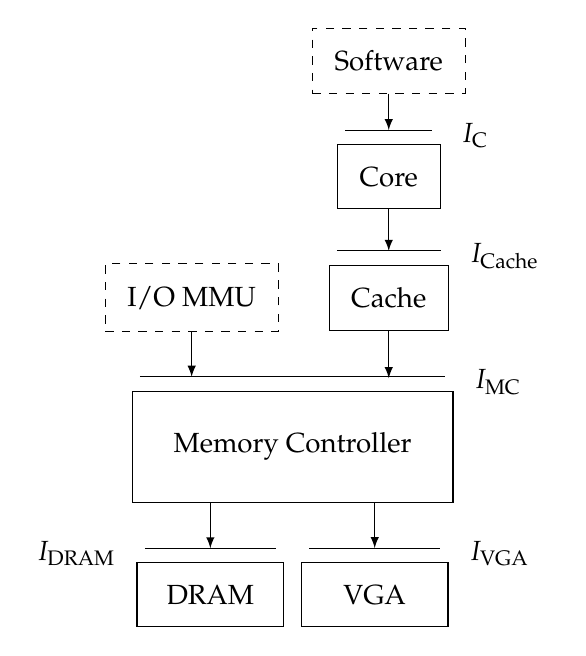
\begin{tikzpicture}
    % Memory Controller
    \node [inner sep=15pt, draw] (MC) {Memory Controller};%
    \draw ([yshift=5pt, xshift=3pt]MC.north west) -- ([yshift=5pt,
    xshift=-3pt]MC.north east);%
    \node [right=4pt of MC.north east, yshift=3pt, text width=0.5cm] (Im)
    {$I_{\mathrm{MC}}$};%
    \node [left=4pt of MC.north west, yshift=3pt, text width=0.5cm] (Im_shadow)
    {};%

    % Cache & IOMMU
    \node [above=30pt of MC] (CIO) {};%
    % -- Cache
    \node [inner sep=8pt, draw, right=13pt of CIO.center] (Cache) {Cache};%
    \draw ([yshift=5pt, xshift=3pt]Cache.north west) -- ([yshift=5pt,
    xshift=-3pt]Cache.north east);%
    \node [right=4pt of Cache.north east, yshift=3pt, text width=0.5cm] (Ic)
    {$I_{\mathrm{Cache}}$};%
    \node [left=4pt of Cache.north west, yshift=3pt, text width=0.5cm]
    (Ic_shadow) {};%
    % -- IOMMU
    \node [inner sep=8pt, draw, dashed, left=5pt of CIO.center] (IOMMU) {I/O
      MMU};%

    % CPU
    \node [inner sep=8pt, draw, above=20pt of Cache] (CPU) {Core};%
    \draw ([yshift=5pt, xshift=3pt]CPU.north west) -- ([yshift=5pt,
    xshift=-3pt]CPU.north east);%
    \node [right=4pt of CPU.north east, yshift=3pt] (Ic) {$I_{\mathrm{C}}$};%

    % Software
    \node [inner sep=8pt, draw, dashed, above=30pt of CPU.center] (S)
    {Software};%

    % Mems
    \node [below=50pt of MC.center] (M) {};%
    % -- DRAM
    \node [inner sep=8pt, draw, left=3pt of M.center, text width=1.3cm, text
    badly centered] (DRAM) {DRAM};%
    \draw ([yshift=5pt, xshift=3pt]DRAM.north west) -- ([yshift=5pt,
    xshift=-3pt]DRAM.north east);%
    \node [left=4pt of DRAM.north west, yshift=3pt, text width=1cm] (Id)
    {$I_{\mathrm{DRAM}}$};%
    % -- VGA
    \node [inner sep=8pt, draw, right=3pt of M.center, text width=1.3cm, text
    badly centered] (VGA) {VGA};%
    \draw ([yshift=5pt, xshift=3pt]VGA.north west) -- ([yshift=5pt,
    xshift=-3pt]VGA.north east);%
    \node [right=4pt of VGA.north east, yshift=3pt, text width=1cm] (Iv)
    {$I_{\mathrm{VGA}}$};%

    % arrows
    \draw [-latex] (CPU.south) -- ([yshift=5pt]Cache.north);%
    \draw [-latex] (S.south) -- ([yshift=5pt]CPU.north);%
    \draw [latex-] ([yshift=5pt]DRAM.north) |- (MC.south);%
    \draw [latex-] ([yshift=5pt]VGA.north) |- (MC.south);%
    \draw [-latex] (IOMMU.south) -- ([yshift=-41pt]IOMMU.north);%
    \draw [-latex] (Cache.south) -- ([yshift=-41pt]Cache.north);
  \end{tikzpicture}

  \caption{Interface-driven modeling of the x86 architecture}
  \label{fig:freespec:interfacedriven}
\end{figure}

We now give an overview of the formalism that we propose to
overcome {\scshape Minx86} limitations, both to model and verify a hardware
architecture.
%
Its key concept is to focus of components \emph{interfaces}, where an interface
is a set of interdependent operations which are expected to produce a value.

\paragraph{Interface and Component}
%
A component is characterized primarily by the interface it exposes to the rest
of the system, and secondarily by its current state and the interfaces it uses
in order to operate.
%
A component receives requests to compute results of operations through its
interface, and sends operations requests to other components it is connected to
\emph{via} their interfaces and waits for their results.

\begin{example}[{\scshape Minx86} as a component-based system]
  Figure~\ref{fig:freespec:interfacedriven} pictures an alternative model to
  {\scshape Minx86}.
  %
  The software components interact with the core \emph{via} its instructions
  set.
  %
  When the core needs to read from or write to memory, it leverages its cache.
  %
  In case of cache miss or cache eviction, the cache interacts with the system
  memory through the memory controller, whose goal is to dispatch memory
  accesses between \emph{e.g.} \ac{dram} and the VGA controller.
  %
  In addition, the memory controller dispatches memory requests coming from
  other sources, for instance an I/O~MMU ---something that we have not taken
  into account in the proofs in Chapter~\ref{chapter:freespec}.
\end{example}

\paragraph{Abstract Specifications}
%
To enable compositional reasoning about component-based systems, we introduce
so-called abstract specifications which are characterized by requirements over
how the interface should be used and requirements over the interface operations
results.

\begin{figure}
  \begin{center}
    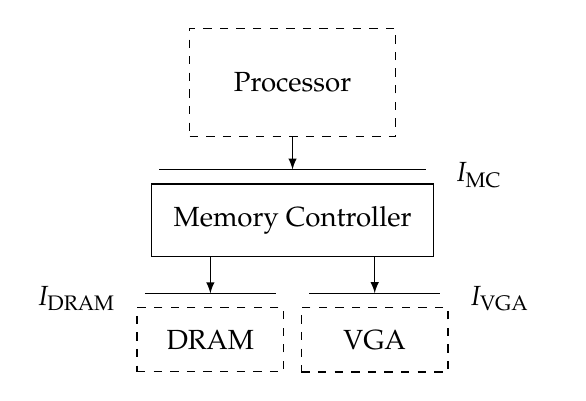
\begin{tikzpicture}
      % Mems
      % -- DRAM
      \node (M) {};%
      \node [inner sep=8pt, dashed, draw, left=3pt of M.center, text
      width=1.3cm, text badly centered] (DRAM) {DRAM};%
      \draw ([yshift=5pt, xshift=3pt]DRAM.north west) -- ([yshift=5pt,
      xshift=-3pt]DRAM.north east);%
      \node [left=4pt of DRAM.north west, yshift=3pt, text width=1cm] (Id)
      {$I_{\mathrm{DRAM}}$};%
      % -- VGA
      \node [inner sep=8pt, dashed, draw, right=3pt of M.center, text
      width=1.3cm, text badly centered] (VGA) {VGA};%
      \draw ([yshift=5pt, xshift=3pt]VGA.north west) -- ([yshift=5pt,
      xshift=-3pt]VGA.north east);%
      \node [right=4pt of VGA.north east, yshift=3pt, text width=1cm] (Iv)
      {$I_{\mathrm{VGA}}$};%

      % Memory Controller
      \node [inner sep=8pt, draw, above=30pt of M.center] (MC) {Memory
        Controller};%
      \draw ([yshift=5pt, xshift=3pt]MC.north west) -- ([yshift=5pt,
      xshift=-3pt]MC.north east);%
      \node [right=4pt of MC.north east, yshift=3pt] (Im) {$I_{\mathrm{MC}}$};%

      % CPU
      \node [inner sep=16pt, draw, dashed, above=30pt of MC.center] (CPU)
      {Processor};%

      % arrows
      \draw [-latex] (CPU.south) -- ([yshift=5pt]MC.north);%
      \draw [latex-] ([yshift=5pt]DRAM.north) |- (MC.south);%
      \draw [latex-] ([yshift=5pt]VGA.north) |- (MC.south);%
    \end{tikzpicture}
  \end{center}

  \caption{The memory controller in isolation}
  \label{fig:freespec:memc}
\end{figure}

\begin{example}[BIOS Isolation]
  We consider one more time the isolation of the \ac{bios} at runtime, thanks to
  the \ac{smm} and the SMRAM.

  The \texttt{SMRAMC} register, exposed by the memory controller, allows the
  \ac{bios} to configure the main access control mechanism which protects the
  content of the SMRAM from the rest of the software stack.
  %
  Using FreeSpec, we can model and verify this access control mechanism in
  isolation, by focusing on the memory controller alone.
  %
  This is achieved by abstracting away the rest of the hardware model, thanks to
  the interfaces exposed and used by the hardware component of interest, as
  pictured in Figure~\ref{fig:freespec:memc}.
  %
  We model the security policy enforced by the mechanism behind the
  \texttt{SMRAMC} register thanks to an abstract specification.
  %
  An abstract specification is a couple of requirements ---over the interface
  users, and over the interface results--- which translates as follows here:
  %
  \begin{itemize}
  \item We forbid unprivileged \IO targeting the SMRAM when the \texttt{SMRAMC}
    register is not correctly configured.
  \item We guarantee that a processor which read the content of the SMRAM while
    in \ac{smm} will get what is has previously written to \ac{smm} while in
    \ac{smm}.
  \end{itemize}
  %
  We can prove the memory controller is correct with respect to this abstract
  specification, meaning if the processor satisfy the requirements over users,
  then the results computed by the memory controller satisfy the requirements
  over results.

  In such a case, the memory controller works as expected, but this does not
  mean that the result alone is sufficient to conclude about the system as a
  whole.
  %
  We still have to prove the premise, \emph{i.e.} that the processor makes a
  correct use of the memory controller interface.
  %
  However, we do not need to use the model of the memory controller to that end,
  we only need to know that it will behave as specified by the abstract
  specification if the processor does too.

  We focus on modeling the processor, made in our example of two components: a
  core and a cache.
  %
  Similarly to what we achieved with the memory controller, we reason about the
  cache in isolation (as pictured with Figure~\ref{fig:freespec:cachec}).
  %
  We want to prove that
  %
  \begin{inparaenum}
  \item the cache makes a correct use of the memory controller interface, that
    is that each uses of the memory controller interface satisfy the appropriate
    requirements, and
  %
  \item it provides similar guarantee to the core.
  \end{inparaenum}

  We proceed by defining a second abstract specification, this time against the
  interface of the cache.
  %
  This additional abstract specification serves two purposes: it restricts how
  the core is allowed to use the cache, and by construction how the cache uses
  the memory controller, but it also formalizes the expectation of the core.

  In this second case, the requirements over the interface results are the same
  as what we already introduced for the memory controller.
  %
  Trying to prove a cache without SMRR can enforce them would uncover the SMRAM
  cache poisoning attack.
\end{example}

\begin{figure}
  \centering
  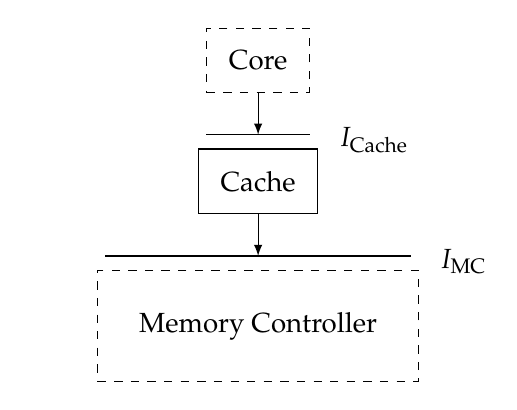
\begin{tikzpicture}
    % Memory Controller
    \node [inner sep=15pt, draw, dashed] (MC) {Memory Controller};%
    \draw ([yshift=5pt, xshift=3pt]MC.north west) -- ([yshift=5pt,
    xshift=-3pt]MC.north east);%
    \node [right=4pt of MC.north east, yshift=3pt, text width=0.5cm] (Im)
    {$I_{\mathrm{MC}}$};%
    \node [left=4pt of MC.north west, yshift=3pt, text width=0.5cm] (Im_shadow)
    {};%

    % Cache
    \node [inner sep=8pt, draw, above=20pt of MC] (Cache) {Cache};%
    \draw ([yshift=5pt, xshift=3pt]Cache.north west) -- ([yshift=5pt,
    xshift=-3pt]Cache.north east);%
    \node [right=4pt of Cache.north east, yshift=3pt, text width=0.5cm] (Ic)
    {$I_{\mathrm{Cache}}$};%
    \node [left=4pt of Cache.north west, yshift=3pt, text width=0.5cm]
    (Ic_shadow) {};%

    % CPU
    \node [inner sep=8pt, draw, above=20pt of Cache, dashed] (CPU) {Core};%

    % arrows
    \draw [-latex] (Cache.south) -- ([yshift=5pt]MC.north); \draw [-latex]
    (CPU.south) -- ([yshift=5pt]Cache.north);
  \end{tikzpicture}

  \caption{The cache in isolation}
  \label{fig:freespec:cachec}
\end{figure}

\subsection*{}

In this Section, we have discussed the limitations of {\scshape Minx86}, and the
strategies that we implemented to mitigate them.
%
This necessary assessment allowed us to propose an alternative formalism to both
model verify the x86 hardware architecture.
%
In the rest of this Chapter, we describe in depth this formalism.

\section{Modeling Programs with Effects}
% ==============================================================================
\label{sec:freespec:specifying}

The first objective of FreeSpec is to incrementally model a complex system, one
component at a time.
%
To do so, we use the key concepts of algebraic effects and effect handlers,
implemented with a variant of the Free monad called the Program monad as defined
in the \texttt{operational} package of Haskell\,\cite{operational}.

This section and the one afterwards proceed through a running example: a
minimalist memory controller, as depicted in Figure~\ref{fig:freespec:memc}.

% pictured in the Figure~\ref{fig:mch-running-example}.
% \begin{figure}
%   \centering \includestandalone[width=.5\textwidth]{running-example}
%
%   \caption{Idealised Memory Controller Hub}
%   \label{fig:mch-running-example}
% \end{figure}

\subsection{Interface of Effects}
% ------------------------------------------------------------------------------

Within a computing system, interconnected components communicate through
interfaces.
%
A component which exhibits an interface receives computational requests from
other components; it handles these requests by computing their results and
sending the latter back to the client component.
%
In FreeSpec, a computational request is modelled with an effect, that is a
symbolic value which describes the request and its potential result.

For $\I$ an interface, we denote by $\Interface{\I}{\mathcal{A}} \subseteq \I$
the subset of effects whose results belong to a set~$\mathcal{A}$.

\begin{example}[Memory Controller Interfaces]
  The VGA and the DRAM controllers exhibit a similar interface which allows for
  reading and writing into a memory region.
  %
  Their interfaces are denoted by $\I_{\mathrm{VGA}}$ and $\I_{\mathrm{DRAM}}$
  respectively.
  %
  Let $\mathpzc{Loc}$ be the set of memory locations and $\mathpzc{Val}$ the set
  of values stored inside the memory region.
  %
  We use the unit value \ac{unit} to model effects without results (similarly to
  the \texttt{void} keyword in an imperative language).
  %
  We define $\I_{\mathrm{DRAM}}$ (respectively $\I_{\mathrm{VGA}}$) with two
  constructors:
  %
  \[
    \begin{array}{rcl}
      \I_{\mathrm{DRAM}}
      & \triangleq
      & \func{Read}_{\mathrm{DRAM}} : \mathpzc{Loc} \rightarrow
        \Interface{\I_{\mathrm{DRAM}}}{\mathpzc{Val}} \\

      & |
      & \func{Write}_{\mathrm{DRAM}} : \mathpzc{Loc} \rightarrow \mathpzc{Val}
        \rightarrow \Interface{\I_{\mathrm{DRAM}}}{\{\ac{unit}\}}
    \end{array}
  \]

  Then,
  $\I_{\mathrm{DRAM}} =
  \Interface{\I_{\mathrm{DRAM}}}{\{\ac{unit}\}}\,\cup\,\Interface{\I_{\mathrm{DRAM}}}{\mathpzc{Val}}$,
  and
  $\func{Read}_{\mathrm{DRAM}}(l) \in
  \Interface{\I_{\mathrm{DRAM}}}{\mathpzc{Val}}$ is an effect that describes a
  memory access to read the value~$v \in \mathpzc{Val}$ stored at the
  location~$l \in \mathpzc{Loc}$.

  The memory controller interface is similar, but it distinguishes between
  privileged and unprivileged accesses.
  %
  It also provides one effect to lock the SMRAM protection mechanism, i.e. it
  enables the SMRAM isolation until the next hardware reset.
  %
  We define the set
  $\mathpzc{Priv}~\triangleq~\{\,\val{privileged}, \val{unprivileged}\,\}$ to
  distinguish between privileged memory accesses made by a processor in \ac{smm}
  and unprivileged accesses made the rest of the time.
  %
  The memory controller interface, denoted by $\I_{\mathrm{MCH}}$, is defined
  with three constructors:
  %
  \[
    \begin{array}{rcl}
      \I_{\mathrm{MCH}}
      & \triangleq
      & \func{Read}_{\mathrm{MCH}} : \mathpzc{Loc} \rightarrow \mathpzc{Priv}
        \rightarrow \Interface{\I_{\mathrm{MCH}}}{\mathpzc{Val}} \\

      & |
      & \func{Write}_{\mathrm{MCH}} : \mathpzc{Loc} \rightarrow \mathpzc{Val}
        \rightarrow \mathpzc{Priv} \rightarrow
        \Interface{\I_{\mathrm{MCH}}}{\{\ac{unit}\}} \\

      & |
      & \func{Lock} : \Interface{\I_{\mathrm{MCH}}}{\{\ac{unit}\}}
    \end{array}
  \]
\end{example}

\subsection{Operational Semantics for Effects}
% -----------------------------------------------------------------------------

An effect corresponds to a computational request made to an implementation of a
given interface.
%
To compute the result of the computational request, we define its
\emph{operational semantics}.
%
Ultimately, we will model a component as an operational semantics for all the
effects of its interface.
%
Since operational semantics are defined using a purely functional language, they
always compute the same result for a given effect, which is inconsistent with
the stateful aspect of hardware components.
%
Thus, an operational semantics produces not only a result, but also a new
operational semantics, which encapsulates the new state of the component.

\begin{definition}[Operational Semantics]
  We write $\Sigma_{\I}$ for the set of operational semantics for a given
  interface $\I$, defined co-inductively as
  %
  \[
    \Sigma_{\I} \triangleq \{\,\sigma\,|\,\sigma : \forall \mathcal{A},
    \Interface{\I}{\mathcal{A}} \rightarrow \mathcal{A} \times \Sigma_{\I} \,\}.
  \]
  %
  An operational semantics~$\sigma \in \Sigma_{\I}$ is a function which, given
  any effect of $\I$, produces both a result which belongs to the expected set
  and a new operational semantics to use afterwards.
\end{definition}

A component may use more than one interface.
%
For instance, the memory controller of our running example can access the system
memory and the memory shared by the VGA controller.
%
But an operational semantics is defined for only one interface.
%
In FreeSpec, we solve this issue by composing interfaces together to create new
ones.

\begin{definition}[Interfaces Composition]
  Let $\I$ and $\J$ be two interfaces. $\oplus$~is the interface composition
  operator, defined with two constructors:
  %
  \[
    \begin{array}{rcl}
      \I \oplus \J
      & \triangleq
      & \func{InL} : \forall \mathcal{A},
        \Interface{\I}{\mathcal{A}} \rightarrow
        \Interface{(\I \oplus \J)}{\mathcal{A}} \\

      & |
      & \func{InR} : \forall \mathcal{A}, \Interface{\J}{\mathcal{A}}
        \rightarrow \Interface{(\I \oplus \J)}{\mathcal{A}}
    \end{array}
  \]
\end{definition}

The resulting interface $\I \oplus \J$ contains the effects of both $\I$ and
$\J$, wrapped into either $\func{InL}$ or $\func{InR}$ constructors.
%
Because constructors images are mutually exclusive\,\footnote{See
  page~\pageref{frontmatter:notations}}, this means we can consider
\( \I \oplus \I \) that is the composition of \( \I \) with itself.
%
This is necessary if we want to be able to reason about a component connected to
two other components which both exhibit the same interface.
%
Besides, \( \oplus \) preserves the effects results, \emph{e.g.} given any
effect \( e \in \I|_{\mathcal{A}} \), then
\( \func{InL(e)} \in \Interface{(\I \oplus \J)}{\mathcal{A}} \).
%
% Notice that this usage of a tagged union allows for composing the same
% interface twice, so a component can use two components which exhibit the same
% interface.

\begin{example}[VGA and DRAM Composition]
  We consider $\I_{\mathrm{DRAM}} \oplus \I_{\mathrm{VGA}}$.
  %
  Then,
  $\func{InL}(\func{Read}_{\mathrm{DRAM}}(l)) \in \Interface{(\I_{\mathrm{DRAM}}
    \oplus \I_{\mathrm{VGA}})}{\mathpzc{Val}}$ is an effect that describes a
  read access targeting the DRAM controller, whereas
  $\func{InR}(\func{Read}_{\mathrm{VGA}}(l)) \in \Interface{(\I_{\mathrm{DRAM}}
    \oplus \I_{\mathrm{VGA}})}{\{\ac{unit}\}}$ is an effect that describes a
  read access targeting the VGA controller.
\end{example}

Using $\oplus$, we can compose several interfaces together.
%
We then need another composition operator, this time for operational semantics.
%
We compose operational semantics together to construct a new operational
semantics for the composed interface.

\begin{definition}[Operational Semantics
  Composition] \label{def:freespec:semantics-composition} Let $\I$ and $\J$ be
  two interfaces, $\sigma_i \in \Sigma_{\I}$ and $\sigma_j \in \Sigma_{\J}$ be
  two operational semantics dedicated to these interfaces.
  %
  We use the $\lambda$-calculus abstraction notation for unnamed functions.
  %
  $\otimes$~is the composition operator for operational semantics, defined as
  \[ \sigma_i \otimes \sigma_j \triangleq \lambda e. \left \{
      \begin{array}{lcl}
        (x, \sigma_i' \otimes \sigma_j) & \text{when} & e =
                                                        \func{InL}(e_i)
                                                        \text{ and }
                                                        \sigma_i(e_i)
                                                        = (x,
                                                        \sigma_i') \\
        (x, \sigma_i \otimes \sigma_j') & \text{when} & e =
                                                        \func{InR}(e_j)
                                                        \text{ and }
                                                        \sigma_j(e_j)
                                                        = (x, \sigma_j')
      \end{array}
    \right.
  \]
\end{definition}

The definition of $\otimes$ has an important impact over what can be specified
in FreeSpec.
%
% When $\sigma_i \otimes \sigma_j$ handles an effect of $\I$, only $\sigma_i$
% ``changes.''
%
Handling an effect of $\I$ (respectively $\J$) does not update $\sigma_j$
(respectively $\sigma_i$).
%
As a consequence, \emph{we cannot specify as-is a graph of components which
  contains a cycle or a diamond}.
%
This is the main limitation of FreeSpec, but its incidence is abated because
computing platforms are often designed as a hierarchical succession of layers.
%
We illustrate it with the four-component system depicted in
Figure~\ref{fig:freespec:diamondpattern}.
%
When \( C_1 \) uses an effect of the interface \( I_{C_2} \), it is possible
that the component \( C_2 \) will itself use an effect of the interface
\( I_{C_4} \).
%
If that happens, the state of the component \( C_4 \), leading the result of the
next effect used by \( C_3 \) to be different, compared it could have been
without the action of \( C_2 \).

\begin{figure}
  \begin{center}
    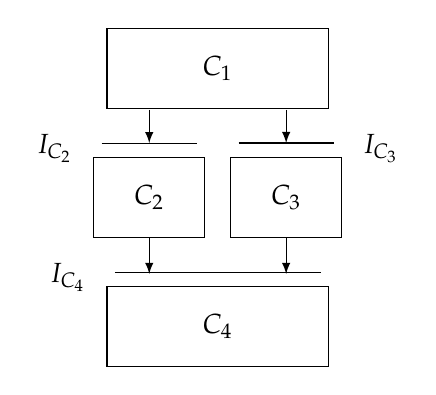
\begin{tikzpicture}
      % c4
      \node [draw, inner sep=10pt, text badly centered, text width=60pt] (C4)
      {$C_4$};%
      \draw ([yshift=5pt, xshift=3pt]C4.north west) -- ([yshift=5pt,
      xshift=-3pt]C4.north east);%
      \node [left=4pt of C4.north west, yshift=3pt] (IC4) {$I_{C_4}$};%

      \node [above=of C4] (Cmid) {};%

      % c2
      \node [draw, text badly centered, text width=20pt, inner sep=10pt,
      left=1pt of Cmid] (C2) {\( C_2 \)};%
      \draw ([yshift=5pt, xshift=3pt]C2.north west) -- ([yshift=5pt,
      xshift=-3pt]C2.north east);%
      \node [left=4pt of C2.north west, yshift=3pt] (IC2) {$I_{C_2}$};%
      % c3
      \node [draw, text badly centered, text width=20pt, inner sep=10pt,
      right=1pt of Cmid] (C3) {\( C_3 \)};%
      \draw ([yshift=5pt, xshift=3pt]C3.north west) -- ([yshift=5pt,
      xshift=-3pt]C3.north east);%
      \node [right=4pt of C3.north east, yshift=3pt] (IC3) {$I_{C_3}$};%

      % c1
      \node [draw, text badly centered, text width=60pt, inner sep=10pt,
      above=of Cmid] (C1) {\( C_1 \)};%

      % arrows
      \draw [-latex] ([yshift=17pt]C2.north) -- ([yshift=5pt]C2.north);%
      \draw [-latex] ([yshift=17pt]C3.north) -- ([yshift=5pt]C3.north);%

      \draw [-latex] (C2.south) -- ([yshift=-13pt]C2.south);%
      \draw [-latex] (C3.south) -- ([yshift=-13pt]C3.south);%
    \end{tikzpicture}
  \end{center}

  \caption{Illustration of the diamond pattern}
  \label{fig:freespec:diamondpattern}
\end{figure}

\GH{Il manque ici une transition pour expliquer pourquoi on a besoin de la monad program. Tu nous parles de çà brusquement et on ne voit pas le lien avec ce qui précède.}

\subsection{The Program Monad}
% -----------------------------------------------------------------------------

Modeling programs with side effects in purely functional languages such as
{\textsc Gallina} (the Coq specification language) or Haskell is usually
achieved thanks to monads\,\cite{hoareetal2001monad}.
%
FreeSpec leverages a variant of the Free monad called the Program
monad\,\cite{operational} to model programs with effects. Operational semantics
play the role of \texttt{operational}\,\cite{operational} interpreters.
%
We write $P_{\I}(\mathcal{A})$ for the set of programs with effects which
belongs to $\I$, modelled thanks to the Program monad, and whose result belongs
to a set $\mathcal{A}$.

\begin{definition}[Program Monad]
  The Program monad is defined with three constructors:
  %
  \[
    \begin{array}{rcl}
      P_{\I}(\mathcal{A})
      & \triangleq
      & \func{Pure} : \mathcal{A} \rightarrow P_{\I}(\mathcal{A}) \\

      & |
      & \func{Bind} : \forall \mathcal{B}, P_{\I}(\mathcal{B}) \rightarrow
        (\mathcal{B} \rightarrow P_{\I}(\mathcal{A})) \rightarrow
        P_{\I}(\mathcal{A}) \\

      & |
      & \func{Request} : \Interface{\I}{\mathcal{A}} \rightarrow
        P_{\I}(\mathcal{A})
    \end{array}
  \]
\end{definition}
%
These constructors allow for the construction of values which act similarly to
abstract syntax trees to model programs with effects.
%
On the one hand, $\func{Pure}$ and $\func{Request}$ are comparable to the leaves
of a syntax tree and model atomic computations; $\func{Pure}$ models local
computations, whereas $\func{Request}$ models deferring a computational request
to a handler and waiting for its result.
%
On the other hand, $\func{Bind}$ (usually written thanks to the infix operator
$\bind$) models the control flow of a program with effects, like the abstract
syntax tree nodes would.
%
It defines how the result of one computation determines the following ones.

\begin{example}[Copy]
  We define
  $\func{copy} : \mathpzc{Loc} \rightarrow \mathpzc{Loc} \rightarrow
  P_{\I_{\mathrm{DRAM}}}(\{\ac{unit}\})$ such that $\func{copy}(l, l')$ models a
  program with effects that returns no result, but copies the value $v$ stored
  at the memory location $l$ inside the memory location $l'$.
  %
  \[ \func{copy}(l, l') \triangleq
    \func{Request}(\func{Read}_{\mathrm{DRAM}}(l)) \bind \lambda
    v. \func{Request}(\func{Write}_{\mathrm{DRAM}}(l', v))
  \]
\end{example}

Given $l \in \mathpzc{Loc}$ and $l' \in \mathpzc{Loc}$, $\func{copy}(l, l')$
symbolically models a program with effects.
%
To assign an interpretation of this program, it must be completed with an
operational semantics which realizes the interface
$\mathcal{I}_{\mathrm{DRAM}}$.

\begin{definition}[Program With Effects
  Realization] \label{def:freespec:realisation} Let $\I$ be an interface,
  $\sigma \in \Sigma_{\I}$ an operational semantics for this interface and
  $\rho \in P_{\I}(\mathcal{A})$ a program with effects which belong to this
  interface.
  %
  $\sigma[\rho] \in \mathcal{A} \times \Sigma_{\I}$ denotes the realization of
  this program by $\sigma$, defined as:
  \[ \sigma[\rho] \triangleq \left\{
      \begin{array}{lcl} (x, \sigma) & \text{if} & \rho =
                                                   \func{Pure}(x) \\
        \sigma(e) & \text{if} & \rho =
                                \func{Request}(e) \\
        \sigma'[f(y)] & \text{if} & \rho =
                                    q \bind f\text{ and }(y, \sigma') = \sigma[q] \\
      \end{array}
    \right.
  \]
\end{definition}

\GH{un petit exemple pour illustrer la précédente définition serait le bienvenu}
\subsection{Components as Programs with Effects}
% -----------------------------------------------------------------------------

With the interfaces, their operational semantics, the $\oplus$ and $\otimes$
operators to compose them and the Program monad to model programs with effects
which belong to these interfaces, we now have all we need to model a given
component which exposes an interface $\I$ and uses another interface $\J$.
%
We proceed with the following steps: modeling the component in terms of programs
with effects, then deriving one operational semantics for $\I$ from these
programs, assuming provided an operational semantics for $\J$. \GH{la tournure "assuming provided an operational semantics for $\J$" me semble bizarre mais je comprends ce que tu as voulu dire. Reformuler?}

The behavior of a component is often determined by a local, mutable state.
%
When it computes the result of a computational request, not only a component may
read its current state; but it can also modify it, for instance to handle the
next computational request differently.
%
This means we have to model the state of a component with a set $\mathcal{S}$ of
symbolic state representations.
%
We map the current state of the component and effects of $\I$ to a program with
effects of $\J$.
%
These programs must compute the effect result and the new state of the
component.

\begin{definition}[Component] \label{def:freespec:component-model} Let $\I$ be
  the interface exhibited by a component and $\J$ the interface it uses.
  %
  Let $\mathcal{S}$ be the set of its states.
  %
  The component $C$, defined in terms of programs with effects of $\J$, is of
  the form
  \[ \forall \mathcal{A}, \Interface{\I}{\mathcal{A}} \rightarrow \mathcal{S}
    \rightarrow P_{\J}(\mathcal{A} \times \mathcal{S}) \]
\end{definition}

Hence, $C$ specifies how the component handles computational requests, both in
terms of computation results and state updates.

\begin{example}[Minimal Memory Controller Model]
  \label{ex:mch-specs}

  Let $C_{\mathrm{MCH}}$ be the memory controller defined in terms of programs
  with effects of $\I_{\mathrm{DRAM}} \oplus \I_{\mathrm{VGA}}$, then
  $C_{\mathrm{MCH}}$ is of the form
  \[
    \forall \mathcal{A}, \Interface{\I_{\mathrm{MCH}}}{\mathcal{A}} \rightarrow
    \mathcal{S}_{\mathrm{MCH}} \rightarrow P_{\I_{\mathrm{DRAM}} \oplus
      \I_{\mathrm{VGA}}}(\mathcal{A} \times \mathcal{S}_{\mathrm{MCH}})
  \] where $\mathcal{S}_{\mathrm{MCH}} \triangleq \{ \val{on}, \val{off} \}$
  means the SMRAM protection is either activated ($\val{on}$) or deactivated
  ($\val{off}$).

  One the one hand, the \func{Lock} effect will activate the isolation mechanism
  of the memory controller, setting its state to $\val{on}$.
  %
  On the other hand, the effects constructed with $\func{Read}_{\mathrm{MCH}}$
  and $\func{Write}_{\mathrm{MCH}}$ will use the current state of the memory
  controller, the privileged parameter of the effect and the memory location of the access
   to determine if it uses the DRAM or the VGA controller.
  %
  By default, it fetches the memory of the DRAM controller, except if all of the three following conditions are satisfied : (1) the  isolation mechanism is activated, (2) the access is unprivileged, and (3) the targeted  memory location belongs to the SMRAM.
  %
  In such a case, it reroutes access to the VGA controller.
\end{example}

A component $C$ defined in terms of programs with effects cannot be used as-is
to compute the result of a given effect.
%
To do that, we need to derive an operational semantics for~$\I$ from $C$.

\begin{definition}[Deriving Operational
  Semantics] \label{def:freespec:derivation} Let $C$ be a component which
  exhibits an interface $\I$, uses an interface~$\J$ and whose states belong to
  $\mathcal{S}$.
  %
  Let $s \in \mathcal{S}$ be the current state of the component and
  $\sigma_j \in \Sigma_{\J}$ be an operational semantics for~$\J$.
  %
  We can derive an operational semantics for $\mathcal{I}$, denoted by
  $\langle C, s, \sigma_j \rangle$, defined as
  \[ \langle C, s, \sigma_j \rangle \triangleq \lambda i. (x, \langle C, s',
    \sigma_j' \rangle) \text{ where } ((x, s'), \sigma_j') = \sigma_j[C (i, s)]
  \]
\end{definition}

\GH{la j'avoue, j'ai décroché sur la définition 6.7. Peut-être qu'un petit exemple ou une petite description de la formule en anglais aiderait à la compréhension.}

% On the one hand, components are defined in terms of programs with effects,
% meaning each component can be modelled independently from the rest of the
% system.
%%
% On the other hand, FreeSpec introduces the mechanism of derivation to
% aggregate these models together.
%
The resulting operational semantics models a system made of interconnected
components, and can then be used to derive another component model into an
operational semantics which models a larger system.
%
For instance, we can proceed with the following steps to comprehensively model
our running example: (i) defining the operational semantics for the DRAM and VGA
controllers; (ii) using these operational semantics to derive an operational
semantics from $C_{\mathrm{MCH}}$.
%
The resulting operational semantics can take part in the derivation of a cache
defined in terms of programs with effects of $\I_{\mathrm{MCH}}$, to model a
larger part of the system pictured in the
Figure~\ref{fig:freespec:interfacedriven}.

\section{Modular Verification of Programs with Effects}
% =============================================================================
\label{sec:freespec:verifying}

The first objective of FreeSpec is to provide the required tools to model each
component of a system independently, and to compose these components to model
the whole system.
%
Its second objective is to verify that the composition of several components
satisfies a set of properties.
%
To achieve that, we introduce the so-called abstract specifications, which
allows for specifying, for each interface, expected properties for the effect
results, independently of any underlying handler.
%
Abstract specifications can be used to emphasize the responsibility of each
component of a system regarding the enforcement of a given security policy.
%
Verifying a component is done against abstract specifications of the interfaces
it directly uses, even if it relies on a security property enforced by a deeper
component in the components graph.
%
In this case, we have to verify that every single component which separate them
preserve this property.
%
This procedure can help to prevent or uncover architectural attacks.

In this section, we proceed with our running example by verifying that the
memory controller correctly isolates the SMRAM.
%
In order to do that, we define an abstract specification which states that
privileged reads targeting the SMRAM returns the value which has previously been
stored by a privileged write. It models the SMRAM isolation: unprivileged writes
cannot tamper with the content of the SMRAM, as read by a privileged CPU.

\subsection{Abstract Specification}
% -----------------------------------------------------------------------------

In FreeSpec, an abstract specification dedicated to an interface $\I$ is
twofold.
%
It defines a precondition over the effects that a caller must satisfy; and, in
return, it specifies a postcondition over the effects results that an
operational semantics must enforce.
%
Since both the precondition and the postcondition may vary in time, we
parameterize an abstraction specification with an abstract state and a step
function to update this state after each effect realization.

\begin{definition}[Abstract Specification] \label{def:freespec:abstract-specs}
  An abstract specification $A$ dedicated to an interface $\I$ is 
  defined as a tuple
  $\langle \Omega, \func{step}, \func{pre}, \func{post} \rangle$ where
  \begin{itemize}
  \item $\Omega$ is a set of abstract states
  \item
    $\func{step} : \forall \mathcal{A}, \Interface{\I}{\mathcal{A}} \rightarrow
    \mathcal{A} \rightarrow \Omega \rightarrow \Omega$ is a transition function
    for the abstract state.
  \item $\func{pre} \subseteq \I \times \Omega$ is the precondition over
    effects, such that $(e, \omega) \in \func{pre}$ if and only if the effect
    $e$ satisfies the precondition parameterized with the abstract state
    $\omega$ (denoted by $\func{pre}(e, \omega)$). \GH{je ne comprends pas le denoted by $\func{pre}(e, \omega)$. Quelle est la différence avec $(e, \omega) \in \func{pre}$?}
  \item
    $\func{post} \subseteq \bigcup_{\mathcal{A}} (\Interface{\I}{\mathcal{A}}
    \times \mathcal{A} \times \Omega)$ is the postcondition over effects
    results, such that $(e, x, \omega) \in \func{post}$ if and only if the
    results $x$ computed for the effects $e$ satisfies the postcondition
    parameterized with the abstract state $\omega$ (denoted by
    $\func{post}(e, x, \omega)$). \GH{idem, je ne comprends pas denoted by
    $\func{post}(e, x, \omega)$}
  \end{itemize}
\end{definition}

By defining an abstract specification of an interface $\I$, it becomes possible
to abstract away the effect handler, i.e. the underlying component.
%
As a consequence, reasoning about a program with effects can be achieved without
the need to look at the effect handlers.
%
An abstract specification is dedicated to one verification problem (in our
context, one security property), and it is possible to define as many
abstract specifications as required.

We write
$\func{run}_{\func{step}} : \forall \mathcal{A}, \Sigma_{\I} \rightarrow
P_{\I}(\mathcal{A}) \rightarrow \Omega \rightarrow (\mathcal{A} \times
\Sigma_{\I} \times \Omega)$ for the function which, in addition to realize a
program with effects, updates an abstract state after each effect.
%
Using $\func{run}_{\func{step}}$, we can determine both the precondition over
effects and the postcondition over effects results while an operational
semantics realizes a program with effects.

\begin{example}[Memory Controller Abstract
  Specification] \label{ex:mch-abs-specs} Let $A_{\mathrm{MCH}}$ be the abstract
  specification such that
  $A_{\mathrm{MCH}} = \langle \Omega_{\mathrm{MCH}}, \func{step}_{\mathrm{MCH}},
  \func{pre}_{\mathrm{MCH}}, \func{post}_{\mathrm{MCH}} \rangle$.
  %
  $A_{\mathrm{MCH}}$ models the following property: ``\emph{privileged reads
    targeting the SMRAM return the value which has been previously stored by a
    privileged write}’’:
  \begin{itemize}
  \item Let $\mathpzc{Smram} \subseteq \mathpzc{Loc}$ be the set of memory
    locations which belong to the SMRAM.  We define
    $\Omega_{\mathrm{MCH}} \triangleq \mathpzc{Smram} \rightarrow
    \mathpzc{Val}$, such that $\omega \in \Omega_{\mathrm{MCH}}$ models a view
    of the SMRAM as exposed by the MCH for privileged reads.
  \item We define $\func{step}_{\mathrm{MCH}}$ which updates the view of the MCH
    (modelled as a function) after each privileged write access targeting any
    SMRAM location $l$, that is
    \[ \func{step}_{\mathrm{MCH}}(e, x, \omega) \triangleq \left\{
        \begin{array}{l}
          \lambda l'.  \text{ (if } l = l' \text{ then } v \text{ else } \omega(l')) \\
          \qquad\ \ \text{ if } e = \func{Write}_{\mathrm{MCH}}(l, v, \val{privileged})
          \text{ and } l \in \mathpzc{Smram} \\
          \omega \qquad \text{ otherwise}
        \end{array}
      \right.
    \]
  \item There is no precondition to the use of the memory controller effects, so
    \[ \forall e \in \I,\forall \omega \in \Omega_{\mathrm{MCH}},
      \func{pre}_{\mathrm{MCH}}(e, \omega) \]
  \item The postcondition enforces that the result $x$ of a privileged read
    targeting the SMRAM ($\func{Read}(l, \val{privileged})$) has to match the
    value stored in $A_{\mathrm{MCH}}$ abstract state, i.e. the expected content
    for this memory location $\omega(l)$.
    \[ \func{post}_{\mathrm{MCH}}(e, x, \omega) \triangleq \forall l \in
      \mathpzc{Loc}, e = \func{Read}_{\mathrm{MCH}}(l, \val{privileged}) \wedge
      l \in \mathpzc{Smram} \Rightarrow x = \omega(l)
    \]
  \end{itemize}
\end{example}

% With an abstract specification
% $\langle \Omega, \func{step}, \func{pre}, \func{post} \rangle$, we can
% transparently update a given abstract state while realizing programs.

\subsection{Compliance and Correctness}
% -----------------------------------------------------------------------------

The verification of a component~$C$, which exhibits $\I$ and uses $\J$, consists
in proving we can derive an operational semantics $\sigma_i$ for $\I$ from an
operational semantics $\sigma_j$ for $\J$.
%
This semantics $\sigma_i$ enforces the postcondition of an abstract
specification $A_{\I}$ dedicated to $\I$ (compliance).
%
As $C$ is defined in terms of programs with effects of $\J$, the latter needs to
make a licit usage of $\J$ with respect to an abstract specification $A_{\J}$
dedicated to $\J$ (correctness).

First, $\sigma_i$ complies with $A_{\I}$ if, (1) given any effect which
satisfies $A_{\I}$ precondition, $\sigma_i$ produces a result which satisfies
its postcondition, and if (2) the new operational semantics $\sigma_i'$ also
complies with $A_{\I}$.
%
The precondition and the postcondition are parameterized by an abstract state,
so is the compliance property.

\begin{definition}[Operational Semantics
  Compliance] \label{def:freespec:compliance} Let $A$ be an abstract
  specification for an interface $\I$, defined as
  $\langle \Omega, \func{step}, \func{pre}, \func{post} \rangle$,
  $\omega \in \Omega$, then $\sigma \in \Sigma_{\I}$ complies with $A$ in
  accordance with $\omega$ (denoted by $\sigma \models A[\omega]$) iff.
  \[ \forall e \in \I, \func{pre}(e, \omega) \Rightarrow \func{post}(e, x,
    \omega) \wedge \sigma' \models A[\func{step}(e, x, \omega)] \text{ where
    }(x, \sigma') = \sigma(e)
  \]
\end{definition}

Secondly, programs with effects of $C$ make a licit usage of an operational
semantics $\sigma_j \in \Sigma_{\J}$ which complies with $A_{\J}$ if they only
use effects which satisfy $A_{\J}$ precondition.
%
As for the compliance property, correctness is parameterized with an abstract
state.

\begin{definition}[Program With Effects
  Correctness] \label{def:freespec:correctness} Let $A$ be an abstract
  specification for an interface $\I$, defined as
  $\langle \Omega, \func{step}, \func{pre}, \func{post} \rangle$,
  $\omega \in \Omega$, and $\rho \in P_{\I}(\mathcal{A})$, then $\rho$ is
  correct with respect to $A$ in accordance with $\omega$ (denoted by
  $A[\omega] \modelssym \rho$), iff.
  \[
    A[\omega] \mathrel{\reflectbox{$\models$}} \rho \triangleq \left\{
      \begin{array}{lcl}
        \text{True} & \text{ if} & \rho = \func{Pure}(x) \\
        \func{pre}(e, \omega) & \text{ if} & \rho = \func{Request}(e) \\
        \forall \sigma \in \Sigma_{\I} \text{ such that } \sigma \models
        A[\omega], & & \\
        \qquad A[\omega] \modelssym q \wedge A[\omega'] \modelssym f(x) & \text{
                                                                          if} & \rho = q \bind f \\
        \text{where }(x, \_, \omega') =
        \func{run}_{\func{step}_{\J}}(\sigma, q, \omega) & \\
      \end{array}
    \right.
  \]
  % \guillaumerk{franchement, le symbole \protect\reflectbox{$\models$} est
  % vraiment trop proche de $\models$. Je comprends l'idée mais c'est source de
  % confusion. Je choisirai un symbol bien discinct.}
\end{definition}

Every local computation ($\func{Pure}$) is correct with respect to $A$ in
accordance with~$\omega$.
%
A computation which uses an effect $e \in \I$ ($\func{Request}$) is correct with
respect to $A$ in accordance with~$\omega$ if and only if $e$ satisfies the
precondition of $A$ for the abstract state $\omega$.
%
Finally, the chaining of two programs with effects ($\func{Bind}$) is correct
with $A$ in accordance with~$\omega$ if the first program is correct with $A$ in
accordance with~$\omega$, and the second program is correct in accordance with
the abstract state reached after the realization of the first program.

Properties, inferred from an abstract specification, of a correct program with
effects only hold if it is realized by a compliant operational semantics.
%
Besides, we prove that correct programs preserve operational semantics
compliance.

\begin{theorem}[Compliance Preservation]
  Let $A$ be an abstract specification dedicated to an interface $\I$, then
  $\sigma$ a compliant operational semantics for $\I$ produces a compliant
  operational semantics $\sigma'$ when it realizes a correct program $\rho$,
  that is
  \[
    \sigma \models A[\omega] \wedge A[\omega] \modelssym \rho \Rightarrow
    \sigma' \models A[\omega'] \text{ where }\func{run}_{\func{step}}(\sigma,
    \rho, \omega) = (x, \sigma', \omega')
  \]
\end{theorem}

As for interfaces (with $\oplus$) and operational semantics (with $\otimes$), we
have also defined an abstract specification composition operator $\odot$.
%
We do not detail its definition in this article, but it has the significant
property to allow for reasoning about the composition of interfaces and
composition of operational semantics.

\begin{theorem}[Congruent Composition]
  Let $\I$ (respectively $\J$) be an interface.
  %
  Let $A_{\I}$ (respectively $A_{\J}$) be an abstract specification and
  $\sigma_i \in \Sigma_{\I}$ (respectively $\sigma_j \in \Sigma_{\J}$) be an
  operational semantics for this interface.
  \[ \sigma_i \models A_{\I}[\omega_i] \wedge \sigma_j \models A_{\J}[\omega_j]
    \Rightarrow \sigma_i \otimes \sigma_j \models (A_{\I} \odot
    A_{\J})[\omega_i, \omega_j]
  \]
\end{theorem}

% \begin{theorem}[Congruent Lifting]
%   Let $\I$ (respectively $\J$) be an interface. Let $A_I$ (respectively $A_J$)
%   be an abstract specification and $\rho_i \in P_{\I}(\mathcal{A})$
%   (respectively $\rho_j \in P_{\J}(\mathcal{A})$) be an effectful computation
%   which uses this interface.
%   \[ A_I[\omega_i] \modelssym \rho_i \Rightarrow A_I \odot A_J [\omega_i,
%     \omega_j] \modelssym \func{liftl}(\rho_i)
%   \]
%   \[ A_J[\omega_j] \modelssym \rho_j \Rightarrow A_I \odot A_J [\omega_i,
%     \omega_j] \modelssym \func{liftr}(\rho_j)
%   \]
% \end{theorem}

With the Compliance Preservation, we know that as long as we follow the abstract
specification precondition related to the effects we use, compliant operational
semantics keep enforcing the postcondition.
%
With the Compliance Preservation and Congruent Composition, we know we can
reason locally, that is component by component.

\subsection{Proofs Techniques to Show Compliance For Components}
% -----------------------------------------------------------------------------

We have dived into the mechanisms which allow for composing together compliant
operational semantics, but little has been said about how to prove the
compliance property to begin with.
%
In a typical FreeSpec use case, operational semantics are not built as-is, but
rather derived from a component model
(Definition~\ref{def:freespec:derivation}).
%
How to prove the resulting operational semantics complies with an abstract
specification depends on how the component is connected to the rest of the
system.
%
We have already discussed the consequences of the operational semantics
composition operator $\otimes$
(Definition~\ref{def:freespec:semantics-composition}).
%
Notably, a graph of components which contains a cycle, a diamond or a forward
edge cannot be easily modelled and verified in FreeSpec.
%
In its current state, FreeSpec provides some theorems to verify the properties
of a component model in terms of an abstract specification, depending on the
composition pattern.

\paragraph{Predicate of Synchronization.}
%
The most favorable scenario consists of one component which uses many
components, and is only used by one other component.
%
Let $\I$ and $\J$ be two interfaces and let $C$, a component with a set of
possible states $\mathcal{S}$, which exhibits $\I$ and uses $\J$.
%
Let $A_{\I}$ be an abstract specification dedicated to $\I$.
%
Deriving an operational semantics from $C$ which complies with $A_{\I}$ in
accordance with $\omega_i \in \Omega_I$ requires to show the existence of
$s \in \mathcal{S} \text{ and }\sigma_j \in \Sigma_{\J}$ such that
\[ \langle C, s, \sigma_j \rangle \models A_{\I}[\omega_i]. \]
%
However, proving this statement would not be very satisfying, as it ties our
verification results to one specific operational semantics $\sigma_j$, and by
extension one specific component.
%
As a consequence, we define an abstract specification $A_{\J}$ to generalize our
statement and abstracting away $\sigma_j$.
%
We now need to prove it exists $\omega_j \in \Omega_{\J}$ such that given an
operational semantics $\sigma_j$ which complies with $A_{\J}$ in accordance with
$\omega_j$, the operational semantics derived from $C$, $s$ and $\sigma_j$
complies with $A_{\I}$ in accordance with $\omega_i$, that is
\[ \forall \sigma_j \in \Sigma_{\J}\text{, }\sigma_j \models A_{\J}[\omega_j]
  \Rightarrow \langle C, s, \sigma_j \rangle \models A_{\I}[\omega_i]
\]

The combinatorial explosion of cases introduced by $\omega_i$, $s$ and
$\omega_j$, modified as the component handles effects, makes inductive reasoning
challenging.
%
The FreeSpec framework provides a useful theorem to address these challenges,
which leverages a so-called predicate of synchronization.
%
The latter is defined by the user on a case-by-case basis, to act as an
invariant for the induction, and a sufficient condition to enforce compliance.

\begin{theorem}[Derivation Compliance] \label{theorem:der-compliance} Let
  $\func{sync}$, a relation between abstract states of $\Omega_{\I}$ and
  $\Omega_\J$ and concrete states of $\mathcal{S}$, be a predicate of
  synchronization.
  %
  Then, it is expected that, $\forall \omega_i \in \Omega_{\I}$,
  $s \in \mathcal{S}$ and $\omega_j \in \Omega_{\J}$ such that
  $\func{sync}(\omega_i, s, \omega_j)$ holds, then
  $\forall \sigma_j \in \Sigma_{\J}$ such that
  $\sigma_j \models A_{\J}[\omega_j]$ and $\forall e \in \I$ such that
  $\func{pre}_{\I}(e, \omega_i)$,
  \begin{enumerate}
  \item $C$ preserves the synchronization of states, that is
    $\func{sync}(\omega_i', s', \omega_j')$
  \item $C$ is defined in terms of programs with effects which are correct with
    respect to $A_{\J}$ in accordance with $\omega_j$, that is
    $A_{\J}[\omega_j] \modelssym C(e, s)$
  \item $C$ computes a result for $e$ which satisfies $A_{\I}$ postcondition,
    that is $\func{post}_{\I}(e, x, \omega_i)$
  \end{enumerate}
  where
  $((x, s'), \sigma_j', \omega_j') = \func{run}_{\func{step}_{\J}}(\sigma_j,
  C(e, s), \omega_j)$ and $\omega_i' = \func{step}_{\I}(e, x, \omega_i)$.

  Should these three properties be verified, then we show that
  \[ \func{sync}(\omega_i, s, \omega_j) \wedge \sigma_j \models A_{\J}[\omega_j]
    \Rightarrow \langle C, s, \sigma_j \rangle \models A_{\I}[\omega_i].
  \]
\end{theorem}

\begin{example}[Memory Controller Compliance]
  We want to prove we can derive an operational semantics from
  $C_{\mathrm{MCH}}$ (Example~\ref{ex:mch-specs}) which complies with
  $A_{\mathrm{MCH}}$ (Example~\ref{ex:mch-abs-specs}).

  We define
  $A_{\mathrm{DRAM}} \triangleq \langle \Omega_{\mathrm{DRAM}},
  \func{step}_{\mathrm{DRAM}}, \func{pre}_{\mathrm{DRAM}},
  \func{post}_{\mathrm{DRAM}} \rangle$ an abstract specification dedicated to
  $\I_{\mathrm{DRAM}}$ to express the following property: ``\emph{a read access
    to a memory location which belongs to the SMRAM return the value which have
    been previously written at this memory location}.'' In particular,
  $\Omega_{\mathrm{DRAM}} = \Omega_{\mathrm{MCH}}$, i.e. they are two views of
  the SMRAM, as exposed by the DRAM controller or by the memory controller.
  %
  In this context, the behaviour of VGA is not relevant. Let $\top$ be the
  abstract specification which has no state and such that its precondition and
  postcondition are always satisfied (meaning every operational semantics always
  complies with it).
  %
  Therefore, the abstract specifications dedicated to the interface used by
  $C_{\mathrm{MCH}}$, that is $\I_{\mathrm{DRAM}} \oplus \I_{\mathrm{VGA}}$, is
  $A_{\mathrm{DRAM}} \odot \top$ whose abstract state is
  $\Omega_{\mathrm{DRAM}}$.

  We define the predicate of synchronization $\func{sync}_{\mathrm{MCH}}$ such
  that
  \[ \func{sync}_{\mathrm{MCH}}(\omega_i, s, \omega_j) \triangleq s = \val{on}
    \wedge \forall l \in \mathpzc{Smram}, \omega_i(l) = \omega_j(l)
  \] Hence, we start our reasoning from a situation where the SMRAM isolation is
  already activated and the states of the two abstract specifications are the
  same, meaning the two views of the SMRAM (as stored in the DRAM, and as
  exposed by the memory controller) coincide.
  %
  We prove $\func{sync}_{\mathrm{MCH}}$ satisfies the three premises of the
  Theorem~\ref{theorem:der-compliance}. We conclude we can derive an operational
  semantics from $C_{\mathrm{MCH}}$ which complies with $A_{\mathrm{MCH}}$.
\end{example}

\paragraph{Predicate of Non-Interference.}
%
Another common composition pattern consists of a component which is used by more
than one other component.
%
FreeSpec provides a theorem which allows for extending the result obtained with
the Theorem~\ref{theorem:der-compliance}, in the specific case where concurrent
accesses do not lead to any abstract state update, and always satisfy the
requirements over effects.
%
This represents an important constraint, but matches realistic use cases.
%
In particular, when hardware components interfaces are very large, two
components are likely to use different classes of effects that do not interfere
with each others.

\begin{definition}[Predicate of Non-Interference]
  Let $\I$ be an interface and
  $A \triangleq \langle \Omega, \func{step}, \mathbb{P}, \mathbb{Q} \rangle$ be
  an abstract specification dedicated to $\I$. Let
  $\func{pnf} : \I \rightarrow \ac{prop}$ be a subset of effects. $\func{pnf}$
  is said to be a predicate of non-interference of $A$ (denoted
  $A \| \func{pnf}$) if and only if \[
    \begin{array}{l}
      \forall \mathcal{A}\text{, } \omega \in \Omega\text{, } i \in
      \Interface{\I}{\mathcal{A}}\text{, }x \in \mathcal{A}\text{, } \\ \qquad
      (\func{pnf}(i) \Rightarrow \mathbb{P}(i, \omega)) \wedge (\func{pnf}(i)
      \wedge \mathbb{Q}(i, x, \omega) \Rightarrow \omega = \func{step}(i, x,
      \omega))
    \end{array}
  \]
\end{definition}

In a similar manner to the predicate of synchronization, FreeSpec provides a
theorem to help and guide the verification work of its users.

\begin{theorem}[Non-Interference and Concurrency]
  Let $\sigma \in \Sigma_{\I}$ be an operational semantics dedicated to
  \( \mathcal{I}\).
  %
  Let \( \func{pnf} : \I \rightarrow \ac{prop} \) be a subset of effects. Let
  \( \sigma\!\!\downarrow\!\!\func{pnf} \) be the operational semantics built
  upon \( \sigma \) which executes arbitrary sequences of effects satisfying
  \func{pnf} between two effects.
  %
  We prove that
  \[
    A \| \func{pnf} \wedge \sigma \models A[\omega] \Rightarrow
    \sigma\!\!\downarrow\!\!\func{pnf} \models A[\omega]
  \]
\end{theorem}

In other words, a second component which only uses the effects that satisfies
$\func{pnf}$ can use the interface concurrently to a component proved to be
correct with respect to \( A \).

\begin{example}[Memory Controller and IOMMU]
  As pictured in Figure\,\ref{fig:freespec:interfacedriven}, the memory
  controller not only arbitrates the memory accesses of the CPU, but also to
  other hardware components (mostly PCI and PCIe devices).
  %
  One possible predicate of non-interference for $A_{\mathrm{MCH}}$ is to deny
  the IOMMU the possibility to perform privileged write, so that only the main
  CPU could do it, that is
  %
  \[
    \func{pnf}_{\mathrm{IOMMU}}(e) \triangleq \forall l \in \mathpzc{Loc}, v \in
    \times \mathpzc{Val}, e \neq \func{Write}_{\mathrm{MCH}}(l, v,
    \texttt{privileged})
  \]
  %
  By definition of \( A_{\mathrm{MCH}} \), and more precisely according to its
  transition function, only privileged write accesses update its abstract state.
  %
  Therefore, we prove
  %
  \[
    \forall \mathcal{A}, \omega \in \Omega_{\mathrm{MCH}}, e \in
    \I|_{\mathrm{\mathcal{A}}}, x \in \mathcal{A},
    \func{pnf}_{\mathrm{IOMMU}}(e) \Rightarrow
    \func{step}_{\mathrm{MCH}}(\omega, e, x, \omega) = \omega
  \]
  %
  Besides, the precondition \( \func{pre}_{\mathrm{MCH}} \) always holds true.

  As a consequence, \( A_{\mathrm{MCH}} \| \func{pnf}_{\mathrm{IOMMU}} \), that
  is \( \func{pnf}_{\mathrm{IOMMU}} \) is a predicate of non-interference of \(
  A_{\mathrm{MCH}} \).
\end{example}

\section{Conclusion}
% =============================================================================
\label{sec:freespec:scale}

For two sections, we have introduced the FreeSpec key definitions and theorems
so that we could model a minimal memory controller component and verify its
properties in the presence of a well-behaving DRAM controller.
%
This example has been driven by a real mechanism commonly found inside x86-based
computing platforms.
%
We now discuss how FreeSpec can be leveraged to model and verify larger systems.
% and limitations we anticipate.

The typical workflow of FreeSpec can be summarized as follows: specifying the
interfaces of a system; modeling the components of the system in terms of
programs with effects of these interfaces; identifying the abstract
specifications which express the requirements over each interface; verifying
each component in terms of compliance with these abstract specifications.

Independent groups of people can use FreeSpec to modularly model and verify a
system, as long as they agree on the interfaces and abstract specifications.
%
If, during the verification process, one group finds out a given interface or
abstract specification needs to be updated, the required modifications may
impact its neighbors.
%
For instance, modeling a x86-based computing system, as pictured in
Figure~\ref{fig:freespec:interfacedriven}, using FreeSpec requires to take into
account the cache, and to verify it complies with an abstract specification
similar to the one defined in Example~\ref{ex:mch-abs-specs}.
%
Thus, FreeSpec could have helped uncover the SMRAM cache poisoning attack
previously mentioned\,\cite{wojtczuk2009smram,duflot2009smram}, and other
similar architectural attacks.

The abstract specifications are defined in terms of interfaces, \emph{i.e.}
independently from components.
%
It has two advantages.
%
First, for a given verification problem modelled with a set of abstract
specifications, two components which exhibit the same interface can be proven to
comply with the same abstract specification.
%
In such a case, we can freely interchange these components, and the verification
results remain true.
%
This is useful to consider the challenge posed by components versioning, i.e. a
new version of a component brings new features which could be leveraged by an
attacker.
%
Then, it is possible to verify a given component in terms of several abstract
specifications.
%
This means we can independently conduct several verification works against the
same component.


\chapter{Conclusion}

%----------------------------------------------------------------------------------------
%	THESIS CONTENT - APPENDICES
%----------------------------------------------------------------------------------------

\appendix % Cue to tell LaTeX that the following "chapters" are Appendices

% Include the appendices of the thesis as separate files from the Appendices folder
% Uncomment the lines as you write the Appendices

\chapter{SpecCert Notations}

\chapter{FreeSpec Notations}

%\input{Appendices/AppendixA}
%\input{Appendices/AppendixB}
%\input{Appendices/AppendixC}

%----------------------------------------------------------------------------------------
%	BIBLIOGRAPHY
%----------------------------------------------------------------------------------------

\printbibliography[heading=bibintoc]

%----------------------------------------------------------------------------------------

\end{document}
